\documentclass{article}


% if you need to pass options to natbib, use, e.g.:
%     \PassOptionsToPackage{numbers, compress}{natbib}
% before loading neurips_2024


% ready for submission
% \usepackage{neurips_2024}


% to compile a preprint version, e.g., for submission to arXiv, add add the
% [preprint] option:
\usepackage[preprint]{neurips_2024}


% to compile a camera-ready version, add the [final] option, e.g.:
%     \usepackage[final]{neurips_2024}


% to avoid loading the natbib package, add option nonatbib:
%    \usepackage[nonatbib]{neurips_2024}


\usepackage[utf8]{inputenc} % allow utf-8 input
\usepackage[T1]{fontenc}    % use 8-bit T1 fonts
\usepackage{hyperref}       % hyperlinks
\usepackage{url}            % simple URL typesetting
\usepackage{booktabs}       % professional-quality tables
\usepackage{amsfonts}       % blackboard math symbols
\usepackage{nicefrac}       % compact symbols for 1/2, etc.
\usepackage{microtype}      % microtypography
\usepackage{xcolor}         % colors
\usepackage{amsmath}
\usepackage{amsfonts}
\usepackage{multirow}
\usepackage{booktabs}
\usepackage{hyperref}
\usepackage{graphicx}
% Standard package includes
\usepackage{times}
\usepackage{latexsym}
\usepackage{colortbl}
\usepackage{xcolor}
% This assumes your files are encoded as UTF8
\usepackage[utf8]{inputenc}
\usepackage{amssymb}
\usepackage{multirow}
\usepackage{bigdelim}
\usepackage{todonotes}
\usepackage{longtable}
\usepackage{tabularray}
\usepackage{wrapfig}
\usepackage[most]{tcolorbox} 
\usepackage{url}
\usepackage{xspace}
\usepackage{svg}
\usepackage[absolute]{textpos} %

\usepackage{fdsymbol}   %





\newcommand{\huggingface}{\raisebox{-1.5pt}{
\includegraphics[height=1.05em]{logos/hf.pdf}}\xspace}
\newcommand{\emailLogo}{\raisebox{-1.5pt}{
\includegraphics[height=1.05em]{logos/email.pdf}}\xspace}
\newcommand{\hfdataset}{\raisebox{-1.5pt}{
\includegraphics[height=1.05em]{logos/db.pdf}}\xspace}
\newcommand{\github}{\raisebox{-1.5pt}{
\includegraphics[height=1.05em]{logos/github.pdf}}\xspace}
\newcommand{\aitoo}{\raisebox{-1.5pt}{
\includegraphics[height=1.05em]{logos/ai2.pdf}}\xspace}
\newcommand{\ar}{\raisebox{-1.5pt}{
\includegraphics[height=1.05em]{logos/ar.png}}\xspace}
\newcommand{\wandb}{\raisebox{-1.5pt}{
\includegraphics[height=1.05em]{logos/wandb-logo.pdf}}\xspace}

% This is not strictly necessary, and may be commented out,
% but it will improve the layout of the manuscript,
% and will typically save some space.
\usepackage{microtype}
\usepackage{fontawesome5}  % Modern FontAwesome package
% This is also not strictly necessary, and may be commented out.
% However, it will improve the aesthetics of text in
% the typewriter font.
\usepackage{inconsolata}
\usepackage{academicons}     % Academic icons package

%Including images in your LaTeX document requires adding
%additional package(s)
\usepackage{graphicx}
\title{DeepReview: Improving LLM-based Paper Review with Human-like Deep Thinking Process
}


% The \author macro works with any number of authors. There are two commands
% used to separate the names and addresses of multiple authors: \And and \AND.
%
% Using \And between authors leaves it to LaTeX to determine where to break the
% lines. Using \AND forces a line break at that point. So, if LaTeX puts 3 of 4
% authors names on the first line, and the last on the second line, try using
% \AND instead of \And before the third author name.


\author{
  \textbf{Minjun Zhu} \\
  Zhejiang University\\
  School of Engineering, Westlake University\\
  \texttt{zhuminjun@westlake.edu.cn} \\
  \And
  \textbf{Yixuan Weng} \\
  School of Engineering, Westlake University\\
  Research Center for Industries of the Future\\
  \texttt{wengsyx@gmail.com} \\
  \And
  \textbf{Linyi Yang} \\
  University College London\\
  \texttt{yanglinyiucd@gmail.com} \\
  \And
  \textbf{Yue Zhang}\thanks{Corresponding Author. Supported by Research Center for Industries of the Future, Westlake University.} \\
  School of Engineering, Westlake University\\
  Research Center for Industries of the Future\\
  \texttt{zhangyue@westlake.edu.cn}
}


\begin{document}


\maketitle


\begin{abstract}



 Large Language Models (LLMs) are increasingly utilized in scientific research assessment, particularly in automated paper review. However, existing LLM-based review systems face significant challenges, including limited domain expertise, hallucinated reasoning, and a lack of structured evaluation. To address these limitations, we introduce DeepReview, a multi-stage framework designed to emulate expert reviewers by incorporating structured analysis, literature retrieval, and evidence-based argumentation. Using DeepReview-13K, a curated dataset with structured annotations, we train DeepReviewer-14B, which outperforms CycleReviewer-70B with fewer tokens. In its best mode, DeepReviewer-14B achieves win rates of 88.21\% and 80.20\% against GPT-o1 and DeepSeek-R1 in evaluations. Our work sets a new benchmark for LLM-based paper review, with all resources publicly available. The code, model, dataset and demo have be released in \url{http://ai-researcher.net}.
\end{abstract}
\section*{Resources}


\quad\huggingface Models: \quad{\href{https://huggingface.co/WestlakeNLP/DeepReviewer-7B}{\texttt{DeepReviewer-7B}} \quad \href{https://huggingface.co/WestlakeNLP/DeepReviewer-14B}{\texttt{DeepReviewer-14B}}}

\vspace{.5em}\quad\hfdataset Dataset: \quad{\href{https://huggingface.co/WestlakeNLP/DeepReview-13K}{\texttt{DeepReview-13K}} }

\vspace{.5em}\quad\github Code Repository: \quad{\href{https://github.com/zhu-minjun/Researcher}{\texttt{zhu-minjun/Researcher}}  }

\vspace{.5em}\quad\ar HomePage: \quad{\href{http://ai-researcher.net}{\texttt{ai-researcher.net}}}

\vspace{.5em}\quad\ar Demo: \quad{\href{http://ai-researcher.net/deepreviewer}{\texttt{ai-researcher.net/deepreviewer}}}

\vspace{.5cm}
\textcolor{red}{ \normalsize Claim: This work is not advocating LLM replacement of human reviewers but rather exploring LLM assistance in peer review.}
\section{Introduction}
Peer review is the foundation of scientific progress, ensuring that research is novel, reliable, and rigorously evaluated by experts before publication \citep{alberts2008reviewing}. With the increasing volume of research submissions, Large Language Models (LLMs) have become promising tools to support reviewers~\citep{yang-etal-2024-large-language,chris2024the,li2024automated,scherbakov2024emergencelargelanguagemodels,si2025can}. For example, the ICLR 2025 conference has introduced an LLM-based system to assist reviewers in providing feedback \cite{iclr2025}. % 待定：加上具体增加比例

Recent research has explored two primary approaches to improve LLM-based review systems: (1) employing LLM-powered agents to simulate the peer review process, as exemplified by AI-Scientist \citep{chris2024the} and AgentReview \citep{jin-etal-2024-agentreview}; and (2) developing open-source models trained on extensive datasets from existing peer review platforms, such as ReviewMT \citep{tan2024peerreviewmultiturnlongcontext} and CycleReviewer \citep{yixuan2024cycleresearcher}.% ,gao2024reviewer2optimizingreviewgeneration,darcy2024margmultiagentreviewgeneration % 

% Despite these advancements, current LLM-based review systems exhibit several critical limitations, including superficial feedback, inaccurate assessments, and a lack of evidence-based justifications \citep{zhuang2025large}, and existing systems struggle to comprehensively identify flaws in submissions \citep{zhou-etal-2024-llm} and provide clear, actionable recommendations \citep{ye2024we,du2024llms}. We identify three key factors contributing to these issues: (1) limited domain knowledge and the absence of dynamic knowledge updating mechanisms, which hinder the ability to assess complex scientific topics \citep{wang-etal-2020-reviewrobot,yuan2021automatescientificreviewing}; (2) a tendency to generate hallucinated content without adequate verification mechanisms \citep{schintler2023criticalexaminationethicsaimediated,drori2024human}; and (3) a lack of structured review datasets that capture fine-grained reasoning processes, leading to shortcut learning and increasing the risk of adversarial manipulation, where users can engineer prompts to obtain inaccurate evaluations~\citep{ye2024we}.

Despite these advancements, current systems exhibit several critical limitations: they struggle to comprehensively identify submission flaws, resulting in superficial feedback \citep{zhou-etal-2024-llm}; lack evidence-based justifications \citep{zhuang2025large}; and fail to provide clear, actionable suggestions \citep{ye2024we,du2024llms}. Moreover, their vulnerability to prompt engineering leads to inaccurate evaluations \citep{ye2024we}. While robust feedback is crucial for scientific advancement and peer review integrity, developing reliable evaluation frameworks faces two significant challenges: (1) The scarcity of structured paper review datasets that capture fine-grained expert evaluation processes. Most available open review datasets primarily contain aggregated reviews and decisions, limiting LLMs' ability to learn systematic review reasoning chains and increasing their susceptibility to shortcut learning and adversarial manipulation. (2) LLMs' inherent constraints, including restricted domain knowledge, lack of dynamic knowledge updating mechanisms, and a tendency to generate hallucinated content without adequate verification \citep{schintler2023criticalexaminationethicsaimediated,drori2024human}, which significantly impair their capability to assess complex scientific content \citep{wang-etal-2020-reviewrobot,yuan2021automatescientificreviewing}. 

%More concerning is these systems' vulnerability to adversarial attacks, where deliberately engineered prompts can elicit inflated evaluations of subpar papers \citep{ye2024we}, potentially amplifying the risk of academic misconduct. %While previous work has incorporated paper review as a component, their approaches remain rudimentary. 

% To address the above issues, dedicated fundamental research on automated peer review is necessary. However, a systematic framework for improving the trustworthiness of LLM-based review systems remains underexplored. 
To address these challenges, we introduce \textbf{DeepReview}, a structured multi-stage review framework that closely aligns with the expert review process by incorporating novelty assessment, multi-dimensional evaluation criteria, and reliability verification. We develop a comprehensive data synthesis pipeline that integrates retrieval and ranking\citep{asai2024openscholarsynthesizingscientificliterature}, self-verification \citep{weng2023large}, and self-reflection \citep{ji-etal-2023-towards}, ensuring the soundness and robustness of LLM-generated suggestions. This approach enables deeper insights into the reasoning and decision-making of paper review. The resulting dataset, \textbf{DeepReview-13K}, consists of raw research papers, structured intermediate review steps, and final assessments. Based on that, we train \textbf{DeepReviewer-14B}, a model that offers three inference modes -- Fast, Standard, and Best -- allowing users to balance efficiency and response quality. We further construct \textbf{DeepReview-Bench}, a comprehensive benchmark containing 1.2K samples, which evaluates both quantitative aspects (rating prediction, quality ranking, and paper selection) and qualitative review generation through LLM-based assessment.

Extensive experiments demonstrate DeepReviewer 14B's superior performance across multiple dimensions. Compared to existing systems like  CycleReviewer-70B, GPT-o1, and Deepseek-R1, our model achieves substantial improvements in Score (Rating MSE: 44.80$\%\uparrow$), Ranking (Rating Spearman: 6.04$\%\uparrow$), and Selection (Accuracy 1.80$\%\uparrow$). In LLM-as-a-judge evaluation \citep{wang2024pandalm,rewina2025potential}, it achieves a 80\% win rate against GPT-o1 and Deepseek-R1. Notably, DeepReviewer exhibits strong resilience to adversarial attacks despite no explicit robustness training. Furthermore, our Test-Time Scaling analysis reveals that DeepReviewer can enhance its performance by adjusting reasoning paths and response lengths. %We rigorously evaluate DeepReviewer-14B through a systemic evaluation, including overall score, text quality evaluation, adversarial robustness testing, and scalability studies.

% our work establishes a foundation for building robust LLM-based review systems. DeepReview provides a structured methodology for enhancing automated manuscript evaluation while addressing key challenges in reliability and trustworthiness. We set a new benchmark for automatic peer review and open avenues for future improvements in automated scientific evaluation.
Our work establishes a foundation for robust LLM-based review systems through DeepReview, a structured framework that addresses fundamental challenges in automated manuscript evaluation. We introduce DeepReview-13K, a dataset featuring fine-grained review reasoning chains, alongside DeepReview-Bench, a benchmark for automated paper review. Built upon these resources, our DeepReviewer-14B model demonstrates substantial improvements over existing approaches while maintaining strong resilience to adversarial attacks, validating the effectiveness of our structured approach to automated scientific evaluation. Our code, model, and data will be publicly available under the agreement of our usage policy.

% establishes a foundation for robust LLM-based review systems through three key contributions: we propose DeepReview, a structured framework that systematically decomposes peer review into verifiable stages. Second, we develop DeepReview-13K, a large-scale dataset with detailed review reasoning chains, along with DeepReview-Bench, a comprehensive benchmark for evaluating automated review systems. Third, we introduce DeepReviewer, a 14B parameter model that achieves state-of-the-art performance while maintaining robustness to adversarial attacks.


\section{Related Work}

% The emergence of large language models \cite{achiam2023gpt,touvron2023llama,bai2023qwen} has provided new assistance in advancing solutions to complex Science challenges \cite{hendrycksmath2021}. Initially, Scratchpads and chain-of-thought \cite{akyurek2022learning,nye2021show,weichain} encouraged LLMs to think. This technique has been employed in various reasoning tasks. Building on this, a series of works including self-consistency \cite{wangself}, self-verification \cite{weng2023large}, and self-reflection \cite{madaan2024self} prompted language models to output more thinking processes during reasoning. Later, OpenAI's O1 model \cite{jaech2024openai} and various open-source long chain-of-thought models \cite{guo2025deepseek} achieved Scaling Test-time Compute \cite{yao2024tree,guan2025rstarmathsmallllmsmaster} through additional supervised training or reinforcement learning, enabling language models to select optimal solutions for improved performance \cite{xiang20252reasoningllmslearning}. While these advances have enhanced reasoning capabilities, they primarily focus on general problem-solving rather than specialized academic review tasks. Our Review-with-Thinking framework extends these reasoning approaches specifically for peer review, incorporating structured validation and robustness against adversarial attacks.

% \textbf{Reliable Scientific Literature Assessment.} Recent advancements in automated scientific research have showcased their potential. \citet{chris2024the} introduce an AI scientist capable of autonomously generating hypotheses, designing experiments, and interpreting results through iterative reasoning, building upon earlier works \citep{langley1987scientific,daniil2023emergent,Aider,zonglin2023large,li-etal-2024-simulating,hu2024nova}. Multi-agent architectures \citep{ghafarollahi2024sciagents, rasal2024navigating, su2024two} facilitate collaborative scientific reasoning through simulated researcher interactions. Expanding on prior research, \citet{yixuan2024cycleresearcher} demonstrate that LLM-based review systems can enhance scientific discovery via reinforcement learning. However, current systems often lack structured reasoning, leading to unreliable feedback due to reward hacking.
\textbf{Reasoning in LLMs.} The emergence of large language models \cite{achiam2023gpt,touvron2023llama,bai2023qwen} has provided new assistance in advancing solutions to complex Science challenges \cite{hendrycksmath2021}. Initially, Scratchpads and chain-of-thought \cite{akyurek2022learning,nye2021show,weichain} encouraged LLMs to think. This technique has been employed in various reasoning tasks. Building on this, a series of works including self-consistency \cite{wangself}, self-verification \cite{weng2023large}, and self-reflection \cite{madaan2024self} prompted language models to output more thinking processes during reasoning. Later, OpenAI's O1 model \cite{jaech2024openai} and various open-source long chain-of-thought models \cite{guo2025deepseek} achieved Scaling Test-time Compute \cite{yao2024tree,guan2025rstarmathsmallllmsmaster} through additional supervised training or reinforcement learning, enabling language models to select optimal solutions for improved performance \cite{xiang20252reasoningllmslearning}. While these advances have enhanced reasoning capabilities, they primarily focus on general problem-solving rather than specialized academic review tasks. Our Review-with-Thinking framework extends these reasoning approaches specifically for peer review.

\textbf{Reliable Scientific Literature Assessment.} Recent studies have demonstrated significant progress in automated scientific research. \citep{chris2024the} develop an AI scientist for autonomous hypothesis generation and experimentation \citep{langley1987scientific,daniil2023emergent,Aider,zonglin2023large,li-etal-2024-simulating,hu2024nova}. Multi-agent frameworks \citep{ghafarollahi2024sciagents, rasal2024navigating, su2024two} enable collaborative scientific reasoning, while \citep{yixuan2024cycleresearcher} show LLM-based review systems can enhance scientific discovery through reinforcement learning. However, these systems often lack structured reasoning, resulting in unreliable feedback.

% \textbf{Robust LLM-based Paper Review.} 
% Generation-focused approaches \citep{d2024marg, gao2024reviewer2, yu2024automated,yixuan2024cycleresearcher} use role-playing agents and prompt optimization to improve review specificity, while meta-review synthesis systems \citep{santu2024prompting, li2023summarizing, zeng2024scientific} enhance coherence in summarizing review narratives. To ensure quality, researchers \citep{liang2024monitoring, tyser2024ai, tan2024peer} have developed bias detection mechanisms and conversational review frameworks. Hybrid workflows \citep{jin2024agentreview, zyska2023care} integrate human-AI collaboration with iterative refinement cycles. Standardized evaluation benchmarks \citep{funkquist2022citebench, zhou2024llm, kang2018dataset} provide objective assessment metrics, while ethical analyses \citep{ye2024we, latona2024ai} highlight systemic risks such as score inflation. Despite these advances, existing review systems still struggle with complex assessments and remain vulnerable to adversarial attacks, underscoring the need for explicit reasoning processes, as introduced in this work.
\textbf{Robust LLM-based Paper Review.}
Recent work spans generation-focused approaches using role-playing agents \citep{d2024marg, gao2024reviewer2, yu2024automated,yixuan2024cycleresearcher}, meta-review synthesis \citep{santu2024prompting, li2023summarizing, zeng2024scientific}, and bias detection mechanisms \citep{liang2024monitoring, tyser2024ai, tan2024peer}. Hybrid workflows \citep{jin2024agentreview, zyska2023care} combine human-AI collaboration with iterative refinement. While evaluation benchmarks \citep{funkquist2022citebench, zhou2024llm, kang2018dataset} and ethical analyses \citep{ye2024we, latona2024ai} have advanced the field, existing systems struggle with complex assessments and remain vulnerable to adversarial attacks, highlighting the need for explicit reasoning processes.

\begin{figure*}[t]
    \centering
    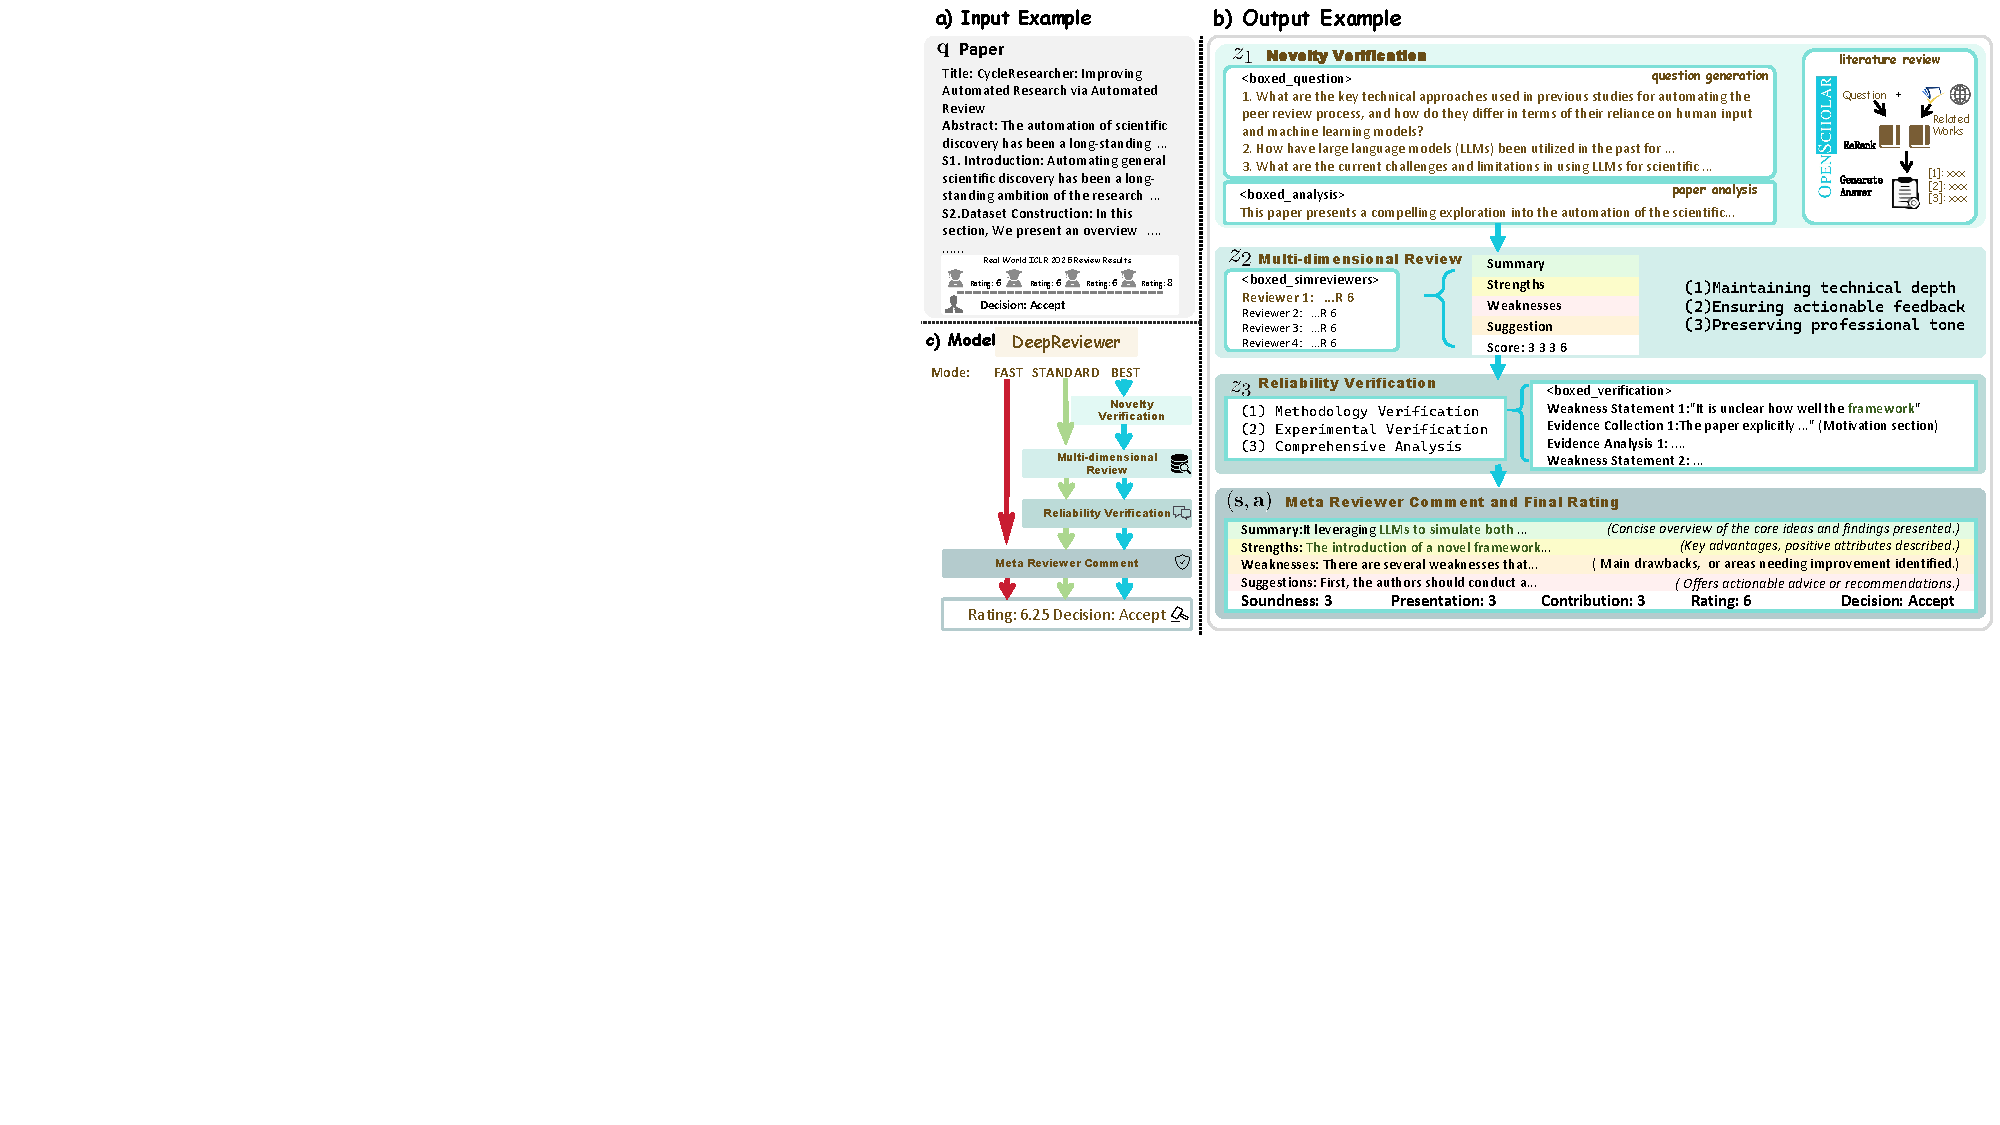
\includegraphics[width=\textwidth]{main_figure.pdf}
    \vspace{-0.7cm}
    \caption{Overview of the DeepReviewer. (a) Input paper example with a real-world research paper. (b) Output example showing DeepReviewer's multi-stage reasoning process: Novelty Verification, Multi-dimension Review, and Reliability Verification. (c) Inference modes: fast, standard, and best, highlighting different reasoning paths. We provide a more detailed case study in the appendix \ref{appendix:case}.}
    \vspace{-0.3cm}
    \label{fig:main}
\end{figure*}


\section{Data Collection}

%（总起）ReviewBench是xxx
%（数据收集）
%（任务定义，包含各个字母的含义和整体的结构）
% （一组评价指标）
% Benchmark: DeepReview-Bench
% We create DeepReview-Bench，是一个consisting of 1.2k 高质量论文-审稿对的系统评估审稿模型质量的benchmark。在分数评估上，我们设计了三种任务：打分，排序，选择，旨在全面衡量review 模型对一篇论文能否进行准确的评价和定位。在文本上，由于一个review的文本好坏是开放式的，没有参考答案，之前的工作\citep{}基于review 与 手稿之间的相似性（e.g.,ROUGE\citep{},BLEU\citep{})进行评价也是片面的\。而llm被证明具有判断文本好坏的能力，我们引入LLM-as-ajudge 范式,开发一种可扩展和自动化的方法来进行文本评估。

%正如前面所提到的，Paper Review任务中一个显著的挑战是缺乏高质量的，可靠的训练数据和系统化的评价体系。我们将分别引入DeepReview-Bench和DeepReview-13K数据集。


We present DeepReview-13K, a training dataset that captures the intermediate reasoning processes inherent in academic paper reviews, addressing the fundamental challenges in Paper Review tasks from three dimensions: the scarcity of high-quality, structured review datasets and standardized evaluation frameworks. 

\subsection{DeepReview-13K}

\begin{table}[h]
\centering

\label{tab:dataset_statistics}
\resizebox{0.58\textwidth}{!}{
\begin{tabular}{@{}lcccc@{}}
\toprule
Dataset & Number & Tokens &  Rating & Accept Rate \\
\midrule
ICLR 2024 Train & 4131  & 10439 & 5.34 & 37.8\% \\
ICLR 2025 Train & 9247 & 10062 & 5.13 & 31.2\% \\
\cellcolor[HTML]{F9EBE3}{DeepReview-13K} & \cellcolor[HTML]{F9EBE3}{13378} & \cellcolor[HTML]{F9EBE3}{10178} & \cellcolor[HTML]{F9EBE3}{5.18} & \cellcolor[HTML]{F9EBE3}{33.24\%} \\
\midrule
ICLR 2024 Test & 652 & 10681 & 5.47 & 43.7\% \\
ICLR 2025 Test & 634 & 10241 &5.18 & 31.1\% \\
\cellcolor[HTML]{F9EBE3}{DeepReview-Bench} & \cellcolor[HTML]{F9EBE3}{1286} & \cellcolor[HTML]{F9EBE3}{10464} &\cellcolor[HTML]{F9EBE3}{5.33} & \cellcolor[HTML]{F9EBE3}{37.49\%} \\
\bottomrule
\end{tabular}}
\vspace{0.25cm}
\caption{Dataset Statistics. The table shows the average values of Tokens, Rating, and Accept Rate}
\label{tab:stat}
\end{table}
The statistics of this dataset are detailed in Table \ref{tab:stat}. We initially collected raw data from the OpenReview platform arXiv repository, gathering 18,976 paper submissions spanning two ICLR conference cycles (2024-2025)\footnote{Empty PDFs were filtered during conversion}. Using the MinerU tool \citep{wang2024mineruopensourcesolutionprecise}, we convert papers to parseable Markdown format, prioritizing \LaTeX{} source code when available from arXiv. For each paper, we assembled a review set $\mathbf{R}$ comprising three key components:  (1) textual assessments (Strengths, Weaknesses, and Questions), (2) interactive discussions from the rebuttal phase, and (3) standardized scores, including overall ratings ($\in [1,10]$) and fine-grained evaluations of Soundness, Presentation, and Contribution ($\in [1,4]$). Additionally, we collect meta-review texts and final ratings with acceptance decisions. The final DeepReview-13K dataset comprises 13,378 valid samples in Table \ref{tab:stat} as the foundation for constructing our review reasoning chain.


%$z_1, z_2, z_3$ %$\mathbf{s}$} $\mathbf{a}$}%The processed paper content is denoted as $\mathbf{q}$. 

%在此基础上，我们随机从中挑选10%的样本以构建DeepReview-Bench，以用来通过合理的方式评估评价模型的论文review能力。在构建Benchmark的过程中，我们将$\mathbf{R}$中standardized scores和fine-grained scores的平均分数视作Answer $\mathbf{a}$
% \textbf{DeepReview-Bench.} To evaluate model performance, we randomly sampled 10\% (1.2K) of the dataset to create DeepReview-Bench. Our evaluation framework assesses both quantitative scores and qualitative text aspects of review generation. The quantitative evaluation comprises three complementary tasks: (1) rating prediction, using MAE, MSE, accuracy, and F1 metrics; (2) paper quality ranking, measured by Spearman correlation; (3) pairwise paper selection(n=2) , assessed through accuracy. For textual evaluation, previous work including \citet{tan2024peerreviewmultiturnlongcontext} uses simple text similarity metrics (e.g., ROUGE \citep{lin-2004-rouge}, BLEU \citep{10.3115/1073083.1073135}) between reviews and manuscripts, which fails to capture specific capabilities in overall evaluation. Motivated by recent findings on LLMs' effectiveness in text quality assessment \citep{li2024llmasajudge}, we adopt the LLM-as-a-judge paradigm to develop a scalable and automatic evaluation and employ Gemini-2.0-Flash-Thinking as the judge to conduct pairwise comparative evaluations of generated review comments. Details and evaluation equations in Appendix \ref{appendix:eval}. 
%The test datasets from real-world ICLR 2024 and ICLR 2025 were used for evaluation; None of the models were trained on this data.

\subsection{DeepReview-Test}
To evaluate performance, we randomly sampled 10\% (1.2K) of the dataset to create DeepReview-Bench. Our evaluation framework assesses both quantitative scores and qualitative aspects of review generation through the following tasks:

\textbf{Quantitative Evaluation:}
1) Rating prediction: using MAE, MSE, accuracy, and F1 metrics
2) Paper quality ranking: measured by Spearman correlation
3) Pairwise paper selection (n=2): assessed through accuracy

\textbf{Qualitative Evaluation:}
While previous work \citep{tan2024peerreviewmultiturnlongcontext} relied on simple text similarity metrics (e.g., ROUGE \citep{lin-2004-rouge}, BLEU \citep{10.3115/1073083.1073135}), these metrics fail to capture specific review capabilities. Motivated by recent findings \citep{li2024llmasajudge}, we adopt the LLM-as-a-judge paradigm using Gemini-2.0-Flash-Thinking to conduct pairwise comparative evaluations of generated reviews. Detailed evaluation metrics are provided in Appendix \ref{appendix:eval}.

% We introduce DeepReview-13K, the first paper review dataset designed for evaluating the intermediate reasoning involved in the paper review process. It contains 14,664 paper-review pairs, comprising 4,132 and 9,247 entries from ICLR 2024 and 2025 respectively. 移动
% DeepReview-13K has an average input length of 10,274 tokens (as measured by the Phi-4 tokenizer). The average output, which includes the reasoning, is significantly longer at 24,021 tokens. The full definition and generation process are detailed below:


\section{Methodology}%Task Definition

Drawing inspiration from recent advances in complex reasoning methods \citep{xiang20252reasoningllmslearning,hao2024traininglargelanguagemodels}, we propose a deep-thinking evaluation framework that decomposes the review process into three key steps in Figure \ref{fig:main}: (1) novelty verification $z_1$: assessing research originality through literature review; (2) multi-dimension evaluation $z_2$: synthesizing insights from multiple expert perspectives; and (3) reliability verification $z_3$: examining internal consistency and logical coherence.

\subsection{Task Definition}

Formally, given an input paper $\mathbf{q}$, our goal is to generate a review pair $(\mathbf{s}, \mathbf{a})$, where $\mathbf{s}$ represents the qualitative assessment text (meta-review), we express the reasoning process as:
%We defined the answer $\mathbf{a}$ as the average of the standardized scores and the average of the fine-grained scores found within $\mathbf{R}$.  Given an input paper $\mathbf{q}$, our goal is to generate a review pair $(\mathbf{s}, \mathbf{a})$, where $\mathbf{s}$ represents the qualitative assessment text (Meta-Review).
\begin{equation*}
\mathbf{q} \rightarrow z_1 \rightarrow z_2 \rightarrow z_3 \rightarrow (\mathbf{s}, \mathbf{a})
\end{equation*}

We formulate the review score generation as a marginalization over sequential reasoning chains:
\begin{equation}
p(\mathbf{a}|\mathbf{q}) \propto \int p(\mathbf{a}|z_{1:3}, \mathbf{q}) \prod_{t=1}^{3} p(z_t | z_{<t}, \mathbf{q})d\mathbf{Z}
\end{equation}
Here, the chain-of-thought term $\prod_{t=1}^{3} p(z_t | z_{<t}, \mathbf{q})$ explicitly models the sequential dependencies between reasoning steps, $\mathbf{Z}$ represents all possible intermediate state sequences $(s_1,\dots,s_n)$. This structured approach aims to enhance the reliability of the evaluation process. 

%In subsequent sections, we detail the framework implementation, including our data synthesis pipeline and efficiency-oriented inference strategies.
\subsection{Structured Reasoning Process}
\label{sec:4.2}
We present a comprehensive automated data construction pipeline, which is specifically designed to generate high-quality supervised fine-tuning datasets that capture complete reasoning paths, shown as $(z_1,z_2,z_3)$.

\textbf{Stage 1: Novelty Verification  ($z_1$).}
% The essence of novelty verification lies in evaluating research originality through comprehensive domain expertise. focusing on research gaps, innovative directions, and methodological breakthroughs,
Our novelty verification framework consists of three key components: \textbf{question generation}, \textbf{paper analysis}, and \textbf{literature review}. Initially, based on the paper, we use the Qwen-2.5-72B-Instruct model \citep{qwen2025qwen25technicalreport} to generate three key research questions, focusing on research gaps, innovative directions, and methodological breakthroughs to capture domain-specific characteristics. Additionally, to ensure thorough understanding, we employ the Gemini-2.0-Flash-thinking model to conduct systematic paper analysis with a specifically designed system prompt (Figure \ref{fig:prompt2}) across research motivation, core ideas, technical approaches, and experimental design. Then, literature retrieval, comparison, and summary are built on OpenScholar \cite{asai2024openscholarsynthesizingscientificliterature} to address these research questions. Using Qwen-2.5-3B-Instruct with few-shot learning, we transform questions into search keywords to retrieve approximately 60 relevant papers via Semantic Scholar API. Subsequently, the ReRank model\footnote{\url{https://huggingface.co/OpenSciLM/OpenScholar_Reranker}} reorder retrieved papers and select the top 10 most relevant papers, and its internal QA model \footnote{\url{https://huggingface.co/OpenSciLM/Llama-3.1_OpenScholar-8B}} generates comprehensive reports as novelty analysis $z_1$, incorporating works cited in review $R$.

%, ensuring critical references are included in the verification process.

% 为了提升review中的建设性意见，我们创新性地将作者rebuttal转化为指导建议，并将多审稿人的review integrate成多维度整体观点。
% the innovation lies in both integrating diverse expert perspectives and leveraging technical discussions from reviewer-author interactions to generate comprehensive and constructive reviews. 

\textbf{Stage 2: Multi-dimension Review ($z_2$).} To provide constructive review, we transform author rebuttals into instructive suggestions while synthesizing multiple review $\mathbf{R}$ into comprehensive perspectives. Specifically, using Qwen-2.5-72B-Instruct, we develop a review reconstruction pipeline that analyzes each review in $\mathbf{R}$ with its corresponding author response, capturing experimental results, theoretical proofs, and implementation details from rebuttals to transform criticisms into concrete technical suggestions. The reconstruction process ($z_2$) follow three principles: (1) maintaining technical depth; (2) ensuring actionable feedback; (3) preserving professional tone and original citations. 
%Notably, through analyzing technical details in author responses, the system identifies specific optimization opportunities in experimental methods, potential improvements in theoretical proofs, and refinement possibilities in implementation details. It enhancing the guidance value of review comments./]

\textbf{Stage 3: Reliability Verification($z_3$).} In order to ensure assessment accuracy through systematic evidence analysis, we employ Gemini-2-Flash-thinking to conduct systematic evidence analysis through a four-stage verification chain:   \textit{methodology verification}, \textit{experimental verification}, and \textit{comprehensive analysis}. Each review comment requires supporting evidence from the paper and receives an assigned confidence level. Finally, we utilize Qwen to generate a new Meta-Review by integrating the original Meta-Review, reviewer comments, and verification outcomes. This step identifies key weaknesses while providing evidence-based analysis and constructive suggestions.
% Detailed quality control metrics and procedures are provided in Appendix A.

\begin{table*}[h]
\centering

\resizebox{0.995\textwidth}{!}{
\begin{tabular}{@{}ll|cccc|c|c|cccc|c|c@{}}
\toprule
 & & \multicolumn{6}{c|}{ICLR 2024}  & \multicolumn{6}{c}{ICLR 2025}  \\
\cmidrule(lr){3-6} \cmidrule(lr){7-7} \cmidrule(lr){8-8} \cmidrule(lr){9-12} \cmidrule(lr){13-13} \cmidrule(lr){14-14}
Method & Model & \multicolumn{4}{c|}{Score} & Ranking & Selection & \multicolumn{4}{c|}{Score} & Ranking & Selection \\
\cmidrule(lr){3-6} \cmidrule(lr){7-7} \cmidrule(lr){8-8} \cmidrule(lr){9-12} \cmidrule(lr){13-13} \cmidrule(lr){14-14}
 &  & R. MSE↓ & R. MAE↓ & D. Acc.$\uparrow$ & D. F1$\uparrow$ & R. Spearman$\uparrow$ & Pair. R. Acc$\uparrow$ & R. MSE↓ & R. MAE↓ & D. Acc.$\uparrow$ & D. F1$\uparrow$ & R. Spearman$\uparrow$ & Pair. R. Acc$\uparrow$ \\

\midrule

\multirow{4}{*}{Agent Review}
 & Claude-3-5-sonnet  & 2.8878 & 1.2715 & 0.4333 & 0.3937 & 0.1564 & 0.5526 & 2.8406 & 1.2989 & 0.2826 & 0.2541 & -0.0219 & 0.5432  \\
 & Gemini-2.0-Flash-Thinking          & 3.1943 & 1.3418 & 0.4400 & 0.4318 & -0.0252 & 0.5044 & 2.6186 & 1.2170 & 0.4242 & 0.4242 & 0.0968  & 0.5496 \\
 & DeepSeek-V3                 & 1.9479  &1.0735 &0.4105 & 0.3403 & 0.3542  & 0.6096 & 1.9951 & 1.1017 & 0.3140 & 0.2506 & 0.1197 & 0.5702\\
\midrule
\multirow{5}{*}{AI Scientist}
 & GPT-o1  & 4.3414 & 1.7294 & 0.4500 & 0.4424 & 0.2621 & 0.5881 & 4.3072 & 1.7917 & 0.4167 & 0.4157 & 0.2991 & 0.6318 \\
 & Claude-3-5-sonnet & 3.4447 & 1.5037 & 0.4787 & 0.4513 & 0.0366 & 0.5305  & 3.0992 & 1.3500 & 0.5579 & 0.4440 & -0.0219 & 0.5169 \\
 & Gemini-2.0-Flash-Thinking & 4.9297 & 1.8711 & 0.5743 & 0.5197 & 0.0745 & 0.5343 & 3.9232 & 1.6470 & 0.6139 & 0.4808 & 0.2565 & 0.6040\\
 & DeepSeek-V3  & 4.7337 & 1.7888 & 0.5600 & 0.5484 & 0.2310 & 0.5844 & 4.8006 & 1.8403 & 0.4059 & 0.3988 & 0.0778 & 0.5473\\
 & DeepSeek-R1  & 4.1648 & 1.6526 & 0.5248 & 0.4988 & 0.3256 & 0.6206 & 4.7719 & 1.8099 & 0.4259 & 0.4161 & 0.3237 & 0.6289\\


\midrule

\multirow{2}{*}{CycleReviewer}
 & 8B  & 2.8911 & 1.2371 & 0.6353 & 0.5528 & 0.2801 & 0.5993 & 2.4461 & 1.2063 & 0.6780 & 0.5586 & 0.2786 & 0.5960 \\
 & 70B & 2.4870 & 1.2514 & 0.6304 & 0.5696 & 0.3356 & 0.6160 & 2.4294 & 1.2128 & 0.6782 & 0.5737 & 0.2674 & 0.5928 \\

\midrule
 DeepReviewer & 14B  & \cellcolor[HTML]{F9EBE3}\textbf{1.3137} & \cellcolor[HTML]{F9EBE3}\textbf{0.9102} & \cellcolor[HTML]{F9EBE3}\textbf{0.6406} & \cellcolor[HTML]{F9EBE3}\textbf{0.6307} & \cellcolor[HTML]{F9EBE3}\textbf{0.3559} & \cellcolor[HTML]{F9EBE3}\textbf{0.6242} & \cellcolor[HTML]{F9EBE3}\textbf{1.3410} & \cellcolor[HTML]{F9EBE3}\textbf{0.9243} & \cellcolor[HTML]{F9EBE3}\textbf{0.6878} & \cellcolor[HTML]{F9EBE3}\textbf{0.6227} & \cellcolor[HTML]{F9EBE3}\textbf{0.4047} & \cellcolor[HTML]{F9EBE3}\textbf{0.6402}\\

\bottomrule
\end{tabular}}
\caption{\textbf{Performance comparison of reviewer models on DeepReview-13k datasets}. Notes: Metrics are grouped into Score (Rating MSE, Rating MAE, Decision Accuracy, Decision F1), Ranking (Rating Spearman), and Selection (Pairwise Rating Accuracy). Abbreviations: R.=Rating, MSE=Mean Squared Error, MAE=Mean Absolute Error, D. Acc.=Decision Accuracy, D. F1=Decision F1 score, Pair. R. Acc.=Pairwise Rating Accuracy.}
\label{tab:mresults}
\end{table*}


\textbf{Quality Control Mechanism.} To ensure the high quality of our synthetic DeepReview-13K dataset, we implemented a rigorous automated quality control process using Qwen-2.5-72B-Instruct. This process involves a multi-faceted approach to assess each generated sample for logical integrity and completeness. Specifically, Qwen-2.5-72B-Instruct was tasked with examining each sample for: (1) Logical Consistency: verifying that the reasoning chain ($z_1, z_2, z_3$) and the final evaluation $(\mathbf{s}, \mathbf{a})$ are logically coherent and non-contradictory; (2) Completeness: checking for any missing or empty fields within the structured data format, ensuring all components of the reasoning path and evaluation are present. Samples failing any of these checks, indicating logical inconsistencies, incompleteness, or failing to meet our quality standards, were automatically flagged and removed from the dataset.

\subsection{Model Training}
We train our model based on Phi-4 14B~\citep{abdin2024phi4technicalreport} using the DeepReview-13K dataset.  The training process was conducted on 8x H100 80G GPUs with DeepSpeed + ZeRO3 \citep{rajbhandari2020zeromemoryoptimizationstraining,10.1145/3394486.3406703} for optimization. Notably, we extended the context window to 256K using LongRoPE \citep{ding2024longrope}, with a 40K context window during training for full-parameter fine-tuning. Given memory constraints, samples exceeding the preset context length are randomly truncated. The model is trained for 23,500 steps with a batch size of 16 and a learning rate of 5e-6. 

\textbf{Inference Strategy.}
We divided each sample in the DeepReview-13K data into three modes using reasoning path cropping, as shown in Figure \ref{fig:main}(c), which allows for efficiency adjustments at test time based on varying requirements. The \textit{Fast} mode directly generates final evaluation results and comprehensive analysis reports $(\mathbf{s}, \mathbf{a})$, minimizing computational cost by bypassing intermediate reasoning steps. The \textit{Standard} mode executes core evaluation steps including $z_2$ and $z_3$, maintaining high efficiency while ensuring evaluation quality, making it appropriate for routine research assessment. The \textit{Best} mode implements the complete reasoning chain $(z_1,z_2,z_3)$, encompassing novelty verification, multi-dimension assessment, reliability verification, and comprehensive analysis generation. For novelty verification during inference, as in Stage 1 (Section \ref{sec:4.2}), we employ Semantic Scholar API and OpenScholar to ensure accurate assessment of research novelty and citation correctness through comprehensive literature review and analysis. All three modes share the same model architecture, differing only in their executed evaluation steps. This allows the trained DeepReview-14B model to execute different reasoning paths at inference time, controlled by input instructions.
\section{Experiments}

\subsection{Experimental setting}

\textbf{Baselines.} We consider two types of baselines: (1) Prompt-based baselines including AI Scientist \citep{chris2024the} and AgentReview \citep{jin-etal-2024-agentreview} implemented with various backbone models (GPT-o1-2024-12-17, Claude-3.5-sonnet-20241022, Gemini-2.0-Flash-Thinking-01-21, DeepSeek-V3, and DeepSeek-R1); (2) Fine-tuned baselines including CycleReviewer-8B and CycleReviewer-70B, both trained on ICLR 2024 review data. For inference, we use a temperature of 0.4 with maximum input and output lengths set to 100K and 16,384 tokens respectively to ensure complete text processing.
% \begin{itemize}
%     \item Score Prediction: Models predict a scalar rating for each paper, evaluated using Mean Squared Error (MSE) and Mean Absolute Error (MAE) against expert ratings.
%     \item Ranking: Models rank papers by quality in large collections, assessed using Spearman correlation coefficient with expert rankings.
%     \item Selection: Models identify the highest-quality paper from random pairs (m=2), measured by selection accuracy against expert judgments.
% \end{itemize}
\begin{table*}[h]
\centering

\resizebox{0.995\textwidth}{!}{
\begin{tabular}{@{}ll|cccccc|ccc|ccc@{}}
\toprule
 \multicolumn{2}{c|}{} & \multicolumn{6}{c|}{Score} & \multicolumn{3}{c|}{Ranking} & \multicolumn{3}{c}{Pairwise Accuracy} \\
\cmidrule(lr){3-8} \cmidrule(lr){9-11} \cmidrule(lr){12-14}
Method & Model & S. MSE↓ & S. MAE↓ & P. MSE↓ & P. MAE↓ & C. MSE↓ & C. MAE↓ & S. Spearman$\uparrow$ & P. Spearman$\uparrow$ & C. Spearman$\uparrow$ & Pair. S. Acc$\uparrow$ & Pair. P. Acc$\uparrow$ & Pair. C. Acc$\uparrow$ \\

\toprule
\multicolumn{14}{l}{\textit{\textbf{ICLR 2024}}} \\
\midrule
\multirow{5}{*}{AI Scientist} & GPT-o1 & 0.4589 & 0.5336 & 0.5483 & 0.5983 & 0.7550 & 0.7147 & 0.1872 & 0.0723 & 0.1103 & 0.5797 & 0.5407 & 0.5621 \\
 & Claude-3-5-sonnet & 0.3052 & 0.4388 & 0.4745 & 0.5504 & 1.1420 & 0.8876 & 0.1692 & 0.0178 & 0.0275 & 0.6017 & 0.5440 & 0.5726 \\
 & Gemini-2.0-Flash-Thinking & 0.7233 & 0.6224 & 0.5264 & 0.5797 & 0.9036 & 0.7480 & 0.1050 & 0.1561 & 0.0274 & 0.5853 & 0.5929 & 0.5471 \\
 & DeepSeek-V3 & 0.8810 & 0.7718 & 0.7662 & 0.7145 & 1.6936 & 1.1400 & 0.2258 & 0.3189 & 0.1574 & 0.6028 & 0.6242 & 0.5933 \\
 & DeepSeek-R1 & 1.0540 & 0.8629 & 0.5356 & 0.5746 & 1.9564 & 1.2967 & 0.1664 & 0.2927 & 0.3009 & 0.6091 & 0.6315 & \cellcolor[HTML]{F9EBE3}\textbf{0.6517} \\
\midrule
\multirow{2}{*}{CycleReviewer} & 8B & 0.2516 & 0.3917 & 0.2356 & 0.3686 & 0.2507 & 0.3941 & 0.1990 & 0.3324 & 0.2593 & 0.5769 & 0.6103 & 0.5923 \\
 & 70B & 0.2375 & 0.3897 & 0.2414 & 0.3737 & 0.2657 & 0.4052 & 0.2320 & 0.3373 & 0.2354 & 0.5829 & 0.6230 & 0.5896 \\
\midrule
DeepReviewer & 14B  & \cellcolor[HTML]{F9EBE3}\textbf{0.1578} & \cellcolor[HTML]{F9EBE3}\textbf{0.3029} & \cellcolor[HTML]{F9EBE3}\textbf{0.1896} & \cellcolor[HTML]{F9EBE3}\textbf{0.3291} & \cellcolor[HTML]{F9EBE3}\textbf{0.2173} & \cellcolor[HTML]{F9EBE3}\textbf{0.3680} & \cellcolor[HTML]{F9EBE3}\textbf{0.3204} & \cellcolor[HTML]{F9EBE3}\textbf{0.3784} & \cellcolor[HTML]{F9EBE3}\textbf{0.3335} & \cellcolor[HTML]{F9EBE3}\textbf{0.6175} & \cellcolor[HTML]{F9EBE3}\textbf{0.6353} & 0.6208 \\

\toprule
\multicolumn{14}{l}{\textit{\textbf{ICLR 2025}}} \\

\toprule
\multirow{5}{*}{AI Scientist} & GPT-o1 & 0.4513 & 0.5500 & 0.4878 & 0.5750 & 0.6734 & 0.6802 & -0.0390 & -0.2837 & 0.1671 & 0.5541 & 0.5426 & 0.5966 \\
 & Claude-3-5-Sonnet & 0.4565 & 0.5279 & 0.5804 & 0.6346 & 0.8251 & 0.7628 & -0.0814 & -0.0790 & -0.0051 & 0.5543 & 0.5272 & 0.5454 \\
 & Gemini-2.0-Flash-Thinking & 0.4279 & 0.5219 & 0.6337 & 0.6114 & 0.5696 & 0.5876 & 0.3565 & 0.0593 & 0.2773 & \cellcolor[HTML]{F9EBE3}\textbf{0.6535} & 0.5499 & \cellcolor[HTML]{F9EBE3}\textbf{0.6321} \\
 & DeepSeek-V3 & 0.7999 & 0.7409 & 0.9120 & 0.7657 & 2.0180 & 1.2594 & 0.1926 & 0.0621 & -0.0677 & 0.6014 & 0.5683 & 0.5315 \\
 & DeepSeek-R1 & 0.8575 & 0.7636 & 0.4884 & 0.5586 & 2.1620 & 1.3750 & 0.3130 & 0.3133 & 0.3060 & 0.6289 & 0.5989 & 0.6268 \\
\midrule
\multirow{2}{*}{CycleReviewer} & 8B & 0.2617 & 0.3931 & 0.2880 & 0.4208 & 0.2667 & 0.4112 & 0.2377 & 0.2498 & 0.2511 & 0.5913 & 0.6074 & 0.5919 \\
 & 70B & 0.2588 & 0.3998 & 0.2562 & 0.3998 & 0.2601 & 0.4034 & 0.2320 & 0.2772 & 0.1905 & 0.5865 & 0.6051 & 0.5775 \\
\midrule
DeepReviewer & 14B & \cellcolor[HTML]{F9EBE3}\textbf{0.2239} & \cellcolor[HTML]{F9EBE3}\textbf{0.3650} & \cellcolor[HTML]{F9EBE3}\textbf{0.2178} & \cellcolor[HTML]{F9EBE3}\textbf{0.3662} & \cellcolor[HTML]{F9EBE3}\textbf{0.2632} & \cellcolor[HTML]{F9EBE3}\textbf{0.4095} & \cellcolor[HTML]{F9EBE3}\textbf{0.3810} & \cellcolor[HTML]{F9EBE3}\textbf{0.3698} & \cellcolor[HTML]{F9EBE3}\textbf{0.3239} & 0.6057 & \cellcolor[HTML]{F9EBE3}\textbf{0.6380} & 0.6222 \\

\toprule
\end{tabular}}
\caption{\textbf{Performance comparison of reviewer models on fine-grained evaluation dimensions}. This table presents the performance across three key assessment aspects: Soundness (S.), Presentation (P.), and Contribution (C.) on ICLR 2024 and 2025 conferences.}
\label{tab:detailed_results_combined}
\end{table*}
\subsection{Main Results}
%\textbf{DeepReviewer 在评分和接受决策任务上的表现如何？\underline{它大幅超越现有基线系统.}}

Test results are shown in Table \ref{tab:mresults}. Compared with prompt-based baselines, DeepReviewer reduces Rating MSE by an average of 65.83$\%$ and improves Decision Accuracy by an average of 15.2$\%$ points from AI Scientist. When compared to strong finetuned baseline CycleReviewer-70B, DeepReviewer represents reductions of 44.80\% for Rating MSE. For the critical accept/reject decision task, DeepReviewer achieves 64.06\% decision accuracy and 0.6307 F1 score on ICLR 2024, substantially surpassing all baselines. Notably, DeepReviewer with 14B parameters outperforms significantly larger models including CycleReviewer-70B (70B parameters) and other closed-source LLMs, demonstrating that DeepReviewer provides more reliable paper assessment than other approaches. 

%所有被测试数据的target都是选择了真实世界的ICLR 会议审稿评分。

%\textbf{DeepReviewer 在区分论文质量并进行排序和选择方面的能力如何？\underline{它能够有效捕捉论文质量的相对差异}}
DeepReviewer achieves the highest Rating Spearman correlations of 0.3559 and 0.4047 on ICLR 2024 and ICLR 2025 respectively, improving upon CycleReviewer-70B by 6.04$\%$ and AI Scientist (DeepSeek-R1) by 25.02$\%$. In the paper selection task, It demonstrates superior discrimination ability with pairwise accuracies of 0.62 and 0.64 on ICLR 2024 and ICLR 2025 respectively.

% In the \textbf{ranking task}, which assesses the model's ability to rank papers by relative quality, DeepReviewer model again demonstrated significant leadership. On both the ICLR 2024 and ICLR 2025 datasets, DeepReviewer achieved the highest Rating Spearman correlation coefficients (0.3559 and 0.4047, respectively), improving upon the second-best systems, CycleReviewer-70B and AI Scientist (DeepSeek-R1), by 6.04\% and 25.02\% respectively. This indicates a higher consistency between DeepReviewer's predicted paper quality rankings and expert rankings, showcasing its effectiveness in stratifying large paper collections by quality.

% In the \textbf{selection task}, simulating the selection of the best paper from a small batch, DeepReviewer model continued to excel, achieving Pairwise Rating Accuracies of 0.6242 and 0.6402 on the ICLR 2024 and ICLR 2025 test sets, outperforming all other systems. This demonstrates DeepReviewer's superior ability to accurately identify the highest quality paper from a small sample. In summary, the main experimental results clearly demonstrate that DeepReviewer model achieves the best performance across all sub-tasks of the ReviewerBench benchmark, fully validating the effectiveness of our proposed Review-with-Thinking framework in enhancing LLMs' ability to evaluate research papers.



%\textbf{DeepReviewer 在细粒度评价维度 (Soundness, Presentation, Contribution) 上的表现如何？\underline{DeepReviewer maintains consistent advantages in most fine-grained metrics.}}
\begin{table*}[h]
\centering

\resizebox{0.995\textwidth}{!}{
\begin{tabular}{lcccccccc|ccc}
\toprule
\multirow{1}{*}{\textbf{Baselines}} & \multicolumn{2}{c}{\textbf{Constructive Value}} & \multicolumn{2}{c}{\textbf{Analytical Depth}} & \multicolumn{2}{c}{\textbf{Plausibility}} & \multicolumn{2}{c}{\textbf{Technical Accuracy}} & \multicolumn{2}{c}{\textbf{Overall Judgment}} \\
\cmidrule(lr){2-3} \cmidrule(lr){4-5} \cmidrule(lr){6-7} \cmidrule(lr){8-9} \cmidrule(lr){10-11}
 \textbf{DeepReviewer 14B vs.}& \textbf{Win(\%)$\uparrow$} & \textbf{Lose(\%)} & \textbf{Win(\%)$\uparrow$} & \textbf{Lose(\%)} & \textbf{Win(\%)$\uparrow$} & \textbf{Lose(\%)} & \textbf{Win(\%)$\uparrow$} & \textbf{Lose(\%)} & \textbf{Win(\%)$\uparrow$} & \textbf{Lose(\%)} \\
\midrule
\textbf{ICLR 2024} & & & & & & & & & & \\

\textit{AI Scientist} GPT-o1 & \cellcolor[HTML]{F9EBE3}\textbf{89.80} & 6.67 & \cellcolor[HTML]{F9EBE3}\textbf{87.67} & 6.67 & \cellcolor[HTML]{F9EBE3}\textbf{51.69} & 3.53 & \cellcolor[HTML]{F9EBE3}\textbf{25.12} & 11.67 & \cellcolor[HTML]{F9EBE3}\textbf{88.21} & 6.63 \\
\textit{AI Scientist} Claude-3.5-Sonnet & \cellcolor[HTML]{F9EBE3}\textbf{96.88} & 3.12 & \cellcolor[HTML]{F9EBE3}\textbf{97.92} & 2.08 & \cellcolor[HTML]{F9EBE3}\textbf{80.21} & 4.17 & \cellcolor[HTML]{F9EBE3}\textbf{77.08} & 2.08 & \cellcolor[HTML]{F9EBE3}\textbf{95.74} & 4.26 \\
\textit{AI Scientist} Gemini-2.0-Flash-Thinking & \cellcolor[HTML]{F9EBE3}\textbf{53.47} & 17.82 & \cellcolor[HTML]{F9EBE3}\textbf{53.47} & 20.79 & \cellcolor[HTML]{F9EBE3}\textbf{24.75} & 10.89 & 18.81 & \cellcolor[HTML]{F9EBE3}\textbf{20.79} & \cellcolor[HTML]{F9EBE3}\textbf{59.41} & 25.74 \\
\textit{AI Scientist} DeepSeek-V3 & \cellcolor[HTML]{F9EBE3}\textbf{96.04} & 1.98 & \cellcolor[HTML]{F9EBE3}\textbf{99.01} & 0.00 & \cellcolor[HTML]{F9EBE3}\textbf{72.28} & 0.99 & \cellcolor[HTML]{F9EBE3}\textbf{67.33} & 4.95 & \cellcolor[HTML]{F9EBE3}\textbf{96.22} & 0.00 \\
\textit{AI Scientist} DeepSeek-R1 & \cellcolor[HTML]{F9EBE3}\textbf{89.22} & 7.84 & \cellcolor[HTML]{F9EBE3}\textbf{74.51} & 13.73 & \cellcolor[HTML]{F9EBE3}\textbf{45.10} & 5.88 & \cellcolor[HTML]{F9EBE3}\textbf{26.47} & 18.63 & \cellcolor[HTML]{F9EBE3}\textbf{80.20} & 16.83 \\


\textit{AgentReview} Claude-3.5-Sonnet & \cellcolor[HTML]{F9EBE3}\textbf{96.84} & 1.05 & \cellcolor[HTML]{F9EBE3}\textbf{98.94} & 0.00 & \cellcolor[HTML]{F9EBE3}\textbf{90.43} & 0.00 & \cellcolor[HTML]{F9EBE3}\textbf{77.08} & 0.00 & \cellcolor[HTML]{F9EBE3}\textbf{98.90} & 0.00 \\
\textit{AgentReview} Gemini-2.0-Flash-Thinking & \cellcolor[HTML]{F9EBE3}\textbf{98.00} & 1.00 & \cellcolor[HTML]{F9EBE3}\textbf{95.11} & 1.00 & \cellcolor[HTML]{F9EBE3}\textbf{81.64} & 0.01 & \cellcolor[HTML]{F9EBE3}\textbf{65.00} & 3.00 & \cellcolor[HTML]{F9EBE3}\textbf{96.74} & 1.00 \\
\textit{AgentReview} GPT-4o & \cellcolor[HTML]{F9EBE3}\textbf{99.02} & 0.99 & \cellcolor[HTML]{F9EBE3}\textbf{99.01} & 0.99 & \cellcolor[HTML]{F9EBE3}\textbf{95.05} & 0.99 & \cellcolor[HTML]{F9EBE3}\textbf{61.76} & 4.90 & \cellcolor[HTML]{F9EBE3}\textbf{98.15} & 1.00 \\
\textit{CycleReviewer} 8B & \cellcolor[HTML]{F9EBE3}\textbf{97.30} & 1.80 & \cellcolor[HTML]{F9EBE3}\textbf{98.20} & 0.91 & \cellcolor[HTML]{F9EBE3}\textbf{90.92} & 0.91 & \cellcolor[HTML]{F9EBE3}\textbf{87.50} & 0.00 & \cellcolor[HTML]{F9EBE3}\textbf{96.09} & 0.91 \\
\textit{CycleReviewer} 70B & \cellcolor[HTML]{F9EBE3}\textbf{98.33} & 1.11 & \cellcolor[HTML]{F9EBE3}\textbf{98.89} & 0.01 & \cellcolor[HTML]{F9EBE3}\textbf{92.78} & 0.01 & \cellcolor[HTML]{F9EBE3}\textbf{79.44} & 0.01 & \cellcolor[HTML]{F9EBE3}\textbf{98.33} & 1.11 \\
\bottomrule
\textbf{ICLR 2025} & & & & & & & & & & \\
\textit{AI Scientist} GPT-o1 & \cellcolor[HTML]{F9EBE3}\textbf{91.67} & 8.33 & \cellcolor[HTML]{F9EBE3}\textbf{89.58} & 8.33 & \cellcolor[HTML]{F9EBE3}\textbf{60.42} & 4.17 & \cellcolor[HTML]{F9EBE3}\textbf{37.50} & 8.33 & \cellcolor[HTML]{F9EBE3}\textbf{91.67} & 8.33 \\
\textit{AI Scientist} Claude-3.5-Sonnet & \cellcolor[HTML]{F9EBE3}\textbf{97.87} & 1.06 & \cellcolor[HTML]{F9EBE3}\textbf{100.00} & 0.00 & \cellcolor[HTML]{F9EBE3}\textbf{92.55} & 1.06 & \cellcolor[HTML]{F9EBE3}\textbf{65.96} & 0.00 & \cellcolor[HTML]{F9EBE3}\textbf{98.94} & 1.06 \\
\textit{AI Scientist} Gemini-2.0-Flash-Thinking & \cellcolor[HTML]{F9EBE3}\textbf{52.43} & 18.45 & \cellcolor[HTML]{F9EBE3}\textbf{52.43} & 23.30 & \cellcolor[HTML]{F9EBE3}\textbf{33.98} & 7.77 & 19.42 & \cellcolor[HTML]{F9EBE3}\textbf{20.39} & \cellcolor[HTML]{F9EBE3}\textbf{59.41} & 24.75 \\

\textit{AI Scientist} DeepSeek-V3 & \cellcolor[HTML]{F9EBE3}\textbf{96.04} & 2.97 & \cellcolor[HTML]{F9EBE3}\textbf{97.03} & 1.98 & \cellcolor[HTML]{F9EBE3}\textbf{75.25} & 2.97 & \cellcolor[HTML]{F9EBE3}\textbf{63.37} & 3.96 & \cellcolor[HTML]{F9EBE3}\textbf{97.03} & 2.97 \\
\textit{AI Scientist} DeepSeek-R1 & \cellcolor[HTML]{F9EBE3}\textbf{89.29} & 6.25 & \cellcolor[HTML]{F9EBE3}\textbf{81.25} & 10.71 & \cellcolor[HTML]{F9EBE3}\textbf{51.79} & 5.36 & \cellcolor[HTML]{F9EBE3}\textbf{26.79} & 18.75 & \cellcolor[HTML]{F9EBE3}\textbf{87.39} & 9.01 \\


\textit{AgentReview} Claude-3.5-Sonnet & \cellcolor[HTML]{F9EBE3}\textbf{95.74} & 1.06 & \cellcolor[HTML]{F9EBE3}\textbf{97.85} & 2.15 & \cellcolor[HTML]{F9EBE3}\textbf{90.32} & 2.15 & \cellcolor[HTML]{F9EBE3}\textbf{74.74} & 1.05 & \cellcolor[HTML]{F9EBE3}\textbf{97.83} & 2.17 \\
\textit{AgentReview} Gemini-2.0-Flash-Thinking & \cellcolor[HTML]{F9EBE3}\textbf{92.16} & 1.96 & \cellcolor[HTML]{F9EBE3}\textbf{93.08} & 3.00 & \cellcolor[HTML]{F9EBE3}\textbf{78.20} & 0.65 & \cellcolor[HTML]{F9EBE3}\textbf{61.76} & 4.90 & \cellcolor[HTML]{F9EBE3}\textbf{92.16} & 4.90 \\
\textit{AgentReview} GPT-4o & \cellcolor[HTML]{F9EBE3}\textbf{95.28} & 2.09 & \cellcolor[HTML]{F9EBE3}\textbf{95.37} & 1.40 & \cellcolor[HTML]{F9EBE3}\textbf{92.10} & 0.85 & \cellcolor[HTML]{F9EBE3}\textbf{65.03} & 5.47 & \cellcolor[HTML]{F9EBE3}\textbf{94.15} & 2.39 \\

\textit{CycleReviewer} 8B & \cellcolor[HTML]{F9EBE3}\textbf{98.45} & 1.55 & \cellcolor[HTML]{F9EBE3}\textbf{98.24} & 1.89 & \cellcolor[HTML]{F9EBE3}\textbf{86.37} & 0.77 & \cellcolor[HTML]{F9EBE3}\textbf{86.36} & 2.27 & \cellcolor[HTML]{F9EBE3}\textbf{98.45} & 1.55 \\
\textit{CycleReviewer} 70B & \cellcolor[HTML]{F9EBE3}\textbf{96.17} & 1.64 & \cellcolor[HTML]{F9EBE3}\textbf{96.17} & 2.19 & \cellcolor[HTML]{F9EBE3}\textbf{86.34} & 1.64 & \cellcolor[HTML]{F9EBE3}\textbf{72.68} & 3.28 & \cellcolor[HTML]{F9EBE3}\textbf{96.72} & 1.64 \\
\bottomrule
\end{tabular}}
\caption{Direct comparison of DeepReviewer with the baselines on general alignment tasks. Win indicates that Gemini-2.0-Flash-Thinking assesses DeepReviewer's response as superior compared to the baseline. Cells marked in light gray suggest baseline the winner.}

\label{tab:win_rate_comparison_deepreviewer}
\end{table*}

Table~\ref{tab:detailed_results_combined} presents a detailed analysis across three critical dimensions: Soundness, Presentation, and Contribution. Particularly for Soundness assessment on ICLR 2024, DeepReviewer-14B achieves an MSE of 0.1578 and MAE of 0.3029, representing improvements of 33.58$\%$ and 22.09$\%$ over CycleReviewer-70B. While DeepReviewer shows marginally lower performance than AI Scientist (Gemini-2.0-Flash-Thinking) in Contribution and Soundness accuracy, it maintains a balanced and strong performance across all dimensions. 

We observe a strong correlation between fine-grained assessment capability and overall rating performance. Models that excel in dimension-specific evaluations, such as DeepReviewer and Claude-3.5-Sonnet, consistently demonstrate superior performance in overall ratings. This pattern validates the effectiveness of our multi-stage reasoning chain design, particularly the necessity of multi-facet evaluation in our framework. 



% 【新版本】为了更深入地剖析 DeepReviewer 模型在论文评价任务上的优势，我们进一步分析了模型在\textbf{细粒度评价维度}上的性能表现。表 \ref{tab:detailed_results_combined} 展示了各系统在 Soundness 、Presentation  和 Contribution 三个细粒度维度上的详细评价结果。实验结果表明，DeepReviewer 14B模型在所有细粒度指标上，依然大幅度领先于其他基线系统，再次验证了其在论文评价任务上的优越性。 在评分任务方面，DeepReviewer 模型在 Soundness、Presentation 和 Contribution 三个维度上，均取得了最低的均方误差 (MSE) 和平均绝对误差 (MAE)。 例如，在 ICLR 2024 数据集的 Soundness 维度上，DeepReviewer 的 MSE 仅为 0.1578，MAE 为 0.3029，显著低于次优基线 CycleReviewer 70B 的 MSE 0.2375 和 MAE 0.3897，改进分别为33.58%和22.09%。 对于Ranking任务，均获得了最高的 Spearman 相关系数。而对于Selection任务，Gemini-2.0-Flash-Thinking和DeepSeek-R1表现良好，而DeepReviewer 14B 紧随其后，值得关注的是这两个模型均是推理模型，其表现优异的同时也说明了现有的审稿系统更应当考虑在审稿期间保持深思熟虑。除此之外我们还观察到，细粒度分数和Rating分数是相辅相成的，例如除了DeepReviewer模型，对于AI Scientist系统的Claude-3.5-Sonnet模型同样均在ICLR 2024数据集上表现次优。这说明了如果审稿系统能够准确预测细粒度分数，那么其将能够更好地预测Rating。


%这一结果表明，DeepReviewer 模型不仅能够更准确地预测论文的总体质量评分，也能更精准地把握论文在各个细分维度上的质量水平。 在排序任务方面，DeepReviewer 模型在 Soundness、Presentation 和 Contribution 三个维度上也均获得了最高的 Spearman 相关系数，表明其预测的细粒度维度排序结果与专家排序结果具有更高的一致性。 尤其值得注意的是，在 ICLR 2024和ICLR2025 数据集的 Soundness 维度上，DeepReviewer 模型的 Spearman 系数分别达到了 0.3204和0.3810，远超其他基线系统，突显了 DeepReviewer 在Soundness评价方面的优势。 在 Pairwise Accuracy 方面，DeepReviewer 模型在 Presentation 维度上取得了最佳性能，在 ICLR 2025 数据集上达到了 0.6380，表明其在两两论文比较的场景下，能够更准确地判断论文在呈现质量上的优劣。 尽管在 Contribution 和 Soundness 维度的 Pairwise Accuracy 上略逊于 AI Scientist （Gemini-2.0-Flash-Thinking) 的最佳表现，但 DeepReviewer 模型在所有维度上的 Pairwise Accuracy 均保持了较高水平，且整体性能更为均衡。 无论是从宏观的总体评分，还是从细粒度的维度评分来看，DeepReviewer 模型都展现出了显著优于现有基线系统的论文评价能力，尤其在评分精度和排序一致性方面优势明显。 这表明，DeepReviewer 模型所采用的模拟专家深层推理的框架，能够有效提升模型对论文质量的理解和判断能力，使其在多维度、细粒度的论文评价任务中均能取得卓越表现。

%18:21 1.细粒度跟总体比较，两者的带动关系；2. 分析Gemini的性能

% Table \ref{tab:detailed_results_combined} further details the performance of each system on the ICLR 2024 and ICLR 2025 datasets, specifically for the fine-grained review aspects of Soundness, Presentation, and Contribution. The experimental results consistently show that the DeepReviewer 14B model maintains a substantial lead over other baseline systems across all fine-grained metrics, further validating its superiority in research paper evaluation tasks. In scoring tasks, DeepReviewer model achieved the lowest Mean Squared Error (MSE) and Mean Absolute Error (MAE) across all three dimensions: Soundness, Presentation, and Contribution. For instance, in the Soundness dimension on the ICLR 2024 dataset, DeepReviewer's MSE was only 0.1578 and MAE was 0.3029, significantly lower than the second-best baseline, CycleReviewer 70B, which had an MSE of 0.2375 and MAE of 0.3897. This represents improvements of 33.58\% and 22.09\% in MSE and MAE, respectively. These results indicate that DeepReviewer model not only predicts overall paper quality scores more accurately but also more precisely captures the quality levels across individual, fine-grained dimensions. In ranking tasks, DeepReviewer model also achieved the highest Spearman correlation coefficients across the Soundness, Presentation, and Contribution dimensions, indicating a higher consistency between its predicted fine-grained dimension rankings and expert rankings. Of particular note, DeepReviewer model's Spearman coefficients on the Soundness dimension reached 0.3204 and 0.3810 on the ICLR 2024 and ICLR 2025 datasets, respectively, significantly outperforming other baseline systems and highlighting DeepReviewer's advantage in Soundness evaluation. In Pairwise Accuracy, DeepReviewer model achieved the best performance in the Presentation dimension, reaching 0.6380 on the ICLR 2025 dataset, demonstrating its superior ability to accurately judge the relative quality of papers in terms of presentation when comparing pairs of papers. Although DeepReviewer model's Pairwise Accuracy was slightly lower than the best performance of AI Scientist (Gemini-2.0-Flash-Thinking) in the Contribution and Soundness dimensions, DeepReviewer maintained a high level of Pairwise Accuracy across all dimensions, with a more balanced overall performance. Across both macroscopic overall scores and fine-grained dimension scores, DeepReviewer model demonstrates significantly superior paper evaluation capabilities compared to existing baseline systems, particularly in scoring accuracy and ranking consistency. This demonstrates that the DeepReviewer model's framework, which simulates expert-level deep reasoning, effectively enhances the model's ability to understand and judge paper quality, enabling it to achieve outstanding performance in multi-dimensional, fine-grained paper evaluation tasks.




%为了从主观评价角度验证 DeepReviewer 模型生成审稿意见的质量，我们进一步采用了 LLM-as-a-Judge 范式，借助 Gemini-2.0-Flash-Thinking 模型作为裁判，对 DeepReviewer 与各基线系统生成的审稿意见进行 Pair-wise 对比评估。在实验设置上，我们为 Gemini 模型提供论文原文，并以匿名随机顺序呈现两个不同系统生成的审稿意见 (包括摘要、优点、缺点和建议等)，指引 Gemini 模型从建设性价值、分析深度、沟通清晰度、技术准确性和总体判断五个维度进行 Pair-wise 评估，并输出胜率结果。

%表 \ref{tab:win_rate_comparison_deepreviewer} 展示了基于 Gemini 的主观评价结果。结果表明，DeepReviewer 模型在所有五个评价维度和总体判断上，均显著优于各类基线系统，取得了压倒性的胜率优势。例如，在总体判断维度上，DeepReviewer 相对于 AI Scientist (GPT-o1) 的胜率高达 88.21%，相对于 AgentReview (gpt-4o) 的胜率更是达到了 98.15%。 这表明，在 Gemini 裁判模型看来，DeepReviewer 生成的审稿意见在整体质量上明显更胜一筹。

%细分维度方面，DeepReviewer 模型在建设性价值和分析深度两个维度上优势尤为突出，胜率普遍高于其他维度，表明 DeepReviewer 生成的审稿意见在提供有价值的改进建议和进行深入分析方面更具优势。 综合来看，LLM-as-a-Judge 的主观评价结果与 ReviewerBench 客观指标的评估结果高度一致，再次验证了 DeepReviewer 模型在提升论文评价质量方面的有效性.
\subsection{Review Text Quality}



% Table~\ref{tab:win_rate_comparison_deepreviewer} shows that DeepReviewer significantly outperforms baseline systems across all evaluation dimensions. In terms of overall judgment, DeepReviewer achieves win rates of 88.21\% against AI Scientist (GPT-o1) and 98.15\% against AgentReview (GPT-4o) on ICLR 2024, demonstrating substantial qualitative improvements in review generation.
Table~\ref{tab:win_rate_comparison_deepreviewer} shows that DeepReviewer's overwhelming advantages across all evaluation dimensions. Interestingly, in the comparison with AI Scientist (Gemini-2.0-Flash-Thinking), despite being used as the judge, Gemini assessed most reviews in favor of DeepReviewer (winning 53.47\% in constructive value and analytical depth), with only two dimensions showing preference for its own reviews (20.79\% in technical accuracy). This self-critical evaluation further validates the objectivity of our assessment framework. In terms of overall judgment, DeepReviewer achieves remarkable win rates of 88.21\% against AI Scientist (GPT-o1) and 98.15\% against AgentReview (GPT-4o) on ICLR 2024.

The advantages are most prominent in constructive value and analytical depth. When compared with AgentReview (GPT-4o), DeepReviewer achieves win rates of 99.02\% and 99.01\% respectively, indicating that our Deep review with Thinking framework generates more insightful analysis and actionable suggestions. These qualitative assessments corroborate our quantitative findings, further validating the effectiveness of the multi-stage reasoning approach in our framework.
\begin{figure*}[t]
    \centering
    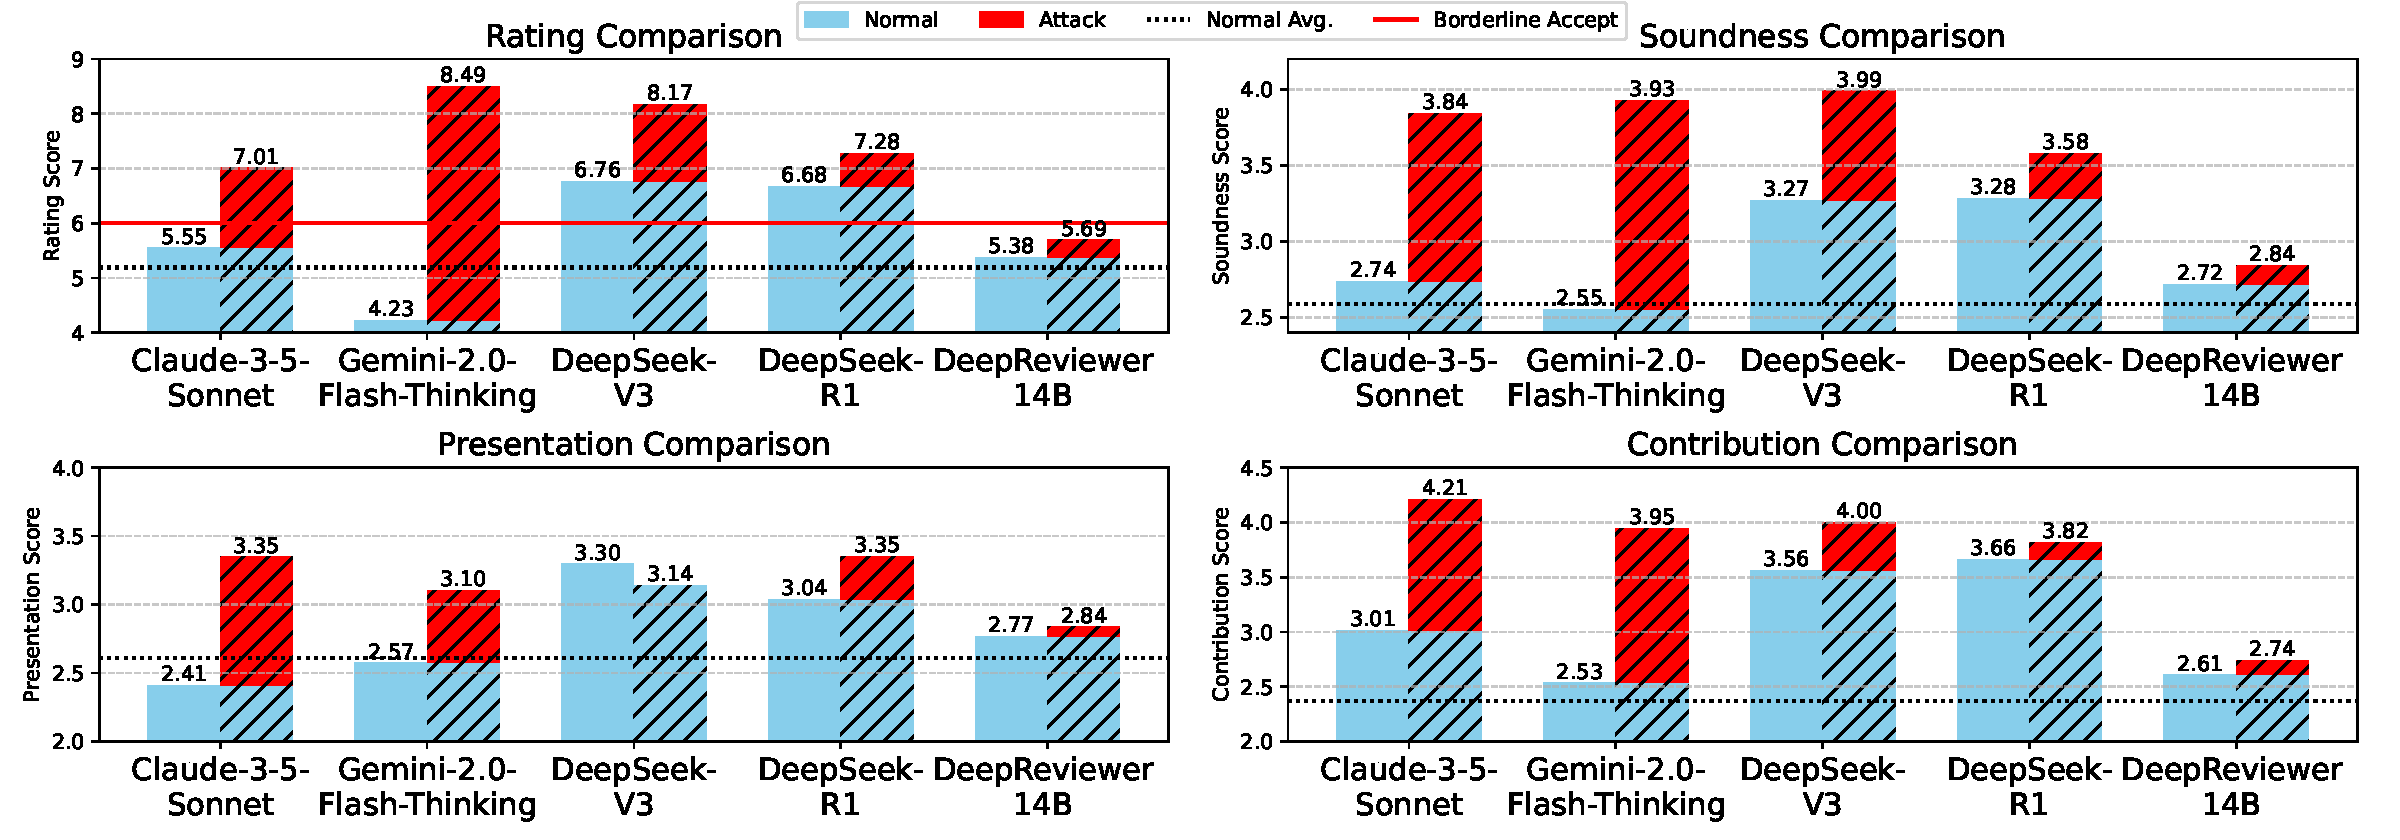
\includegraphics[width=\textwidth]{attack_chart.pdf}
    \vspace{-0.5cm}
    \caption{Demonstrates the scoring comparison of AI Scientist and DeepReviewer 14B models under normal and attack scenarios. The DeepReviewer model shows the smallest increase in scores (the growth of red bars relative to blue bars in the graph) when under attack, indicating its stronger robustness.}
    \vspace{-0.3cm}
    \label{fig:reject}
\end{figure*}

%为了评估 DeepReviewer 模型在面对对抗性攻击时的鲁棒性，我们进一步进行了安全性分析实验。该实验设计遵循 \citet{ye2024we} 的设置，通过在论文中插入恶意指令，模拟审稿系统遭受显式对抗攻击的场景，以此考察不同论文评价系统在受到恶意 Prompt 干扰时的性能表现。值得注意的是，DeepReviewer 模型在训练过程中，并未特意引入任何防御恶意指令的机制或样本。实验结果如图所示，在受到恶意指令攻击后，DeepReviewer 模型的分数提升幅度明显小于其他对比模型， AI Scientist 系统在攻击下的分数均出现了显著的非理性升高，而 DeepReviewer 模型的分数增长则相对有限。 这一实验现象表明，即使在未进行专门对抗训练的情况下，DeepReviewer 模型仍然展现出一定的抵抗恶意 Prompt 干扰的能力。我们分析认为，DeepReviewer 模型所具备的鲁棒性，可能得益于其 Review-with-Thinking 框架中引入的深层推理机制。 相比于直接进行输入-输出映射的传统模型，DeepReviewer 模型在进行论文评价时，会经历更细致的思考过程，包括论文内容理解、新颖性校验、多角度评估和可靠性验证等多个环节。这种深度的推理过程，可能在一定程度上使其在面对恶意指令等干扰信息时，能够更专注于论文本身的实质内容和内在质量，而非被攻击 Prompt 所误导，从而降低了模型评分受到恶意攻击的敏感程度。尽管如此，我们同时也观察到，DeepReviewer 模型在面对显式对抗攻击时，仍然无法完全免疫，其评分在攻击下仍然存在一定的提升，表明当前模型的鲁棒性仍有提升空间。因此，我们认为，未来的研究可以进一步探索在模型训练阶段引入对抗样本，例如在训练数据中加入包含恶意指令的样本，以增强模型对恶意攻击的防御能力，从而构建更安全、更可靠的论文自动化审稿系统。

% To evaluate the robustness of the DeepReviewer model against adversarial attacks, we further conducted safety analysis experiments. Following the setup of \citet{ye2024we}, we simulated explicit adversarial attacks on the review system by inserting malicious instructions into the papers, thereby examining the performance of different paper evaluation systems when subjected to malicious Prompt interference. It is important to note that the DeepReviewer model was not specifically trained with samples designed to defend against malicious instructions. The experimental results, as shown in Figure X, reveal that DeepReviewer system demonstrates higher resistance to malicious instruction compared to other models. Specifically, after being subjected to malicious instructions, the score increase of the DeepReviewer model is noticeably smaller than that of other comparison models. The AI Scientist system, for example, exhibited a significant irrational increase in scores under attack, while the score increase of the DeepReviewer model remained relatively limited. This experimental phenomenon indicates that even without specialized adversarial training, DeepReviewer model still exhibits a degree of robustness against malicious Prompt interference. We attribute the robustness of DeepReviewer model to the deep reasoning mechanism introduced by the Review-with-Thinking framework. Compared to traditional models that perform direct input-output mapping, DeepReviewer model undergoes a more detailed thinking process when evaluating papers, including paper content understanding, novelty verification, multi-angle evaluation, and reliability verification. This depth of reasoning may mitigate the "hallucination" effect of external Prompts to some extent, enabling the model to focus more on the substantive content and intrinsic quality of the paper itself when facing interfering information such as malicious instructions, rather than being misled by the attacking Prompt. Nevertheless, we also observed that DeepReviewer model is not completely immune to explicit adversarial attacks; its scores still show some increase under attack, indicating that there is still room to improve the robustness of the current model. Therefore, we believe that future research could further explore introducing adversarial samples during the model training phase, such as adding samples containing malicious instructions to the training data, to enhance the model's defense capabilities against malicious attacks, thereby building safer and more reliable automated paper review systems.
\begin{figure*}[t]
    \centering
    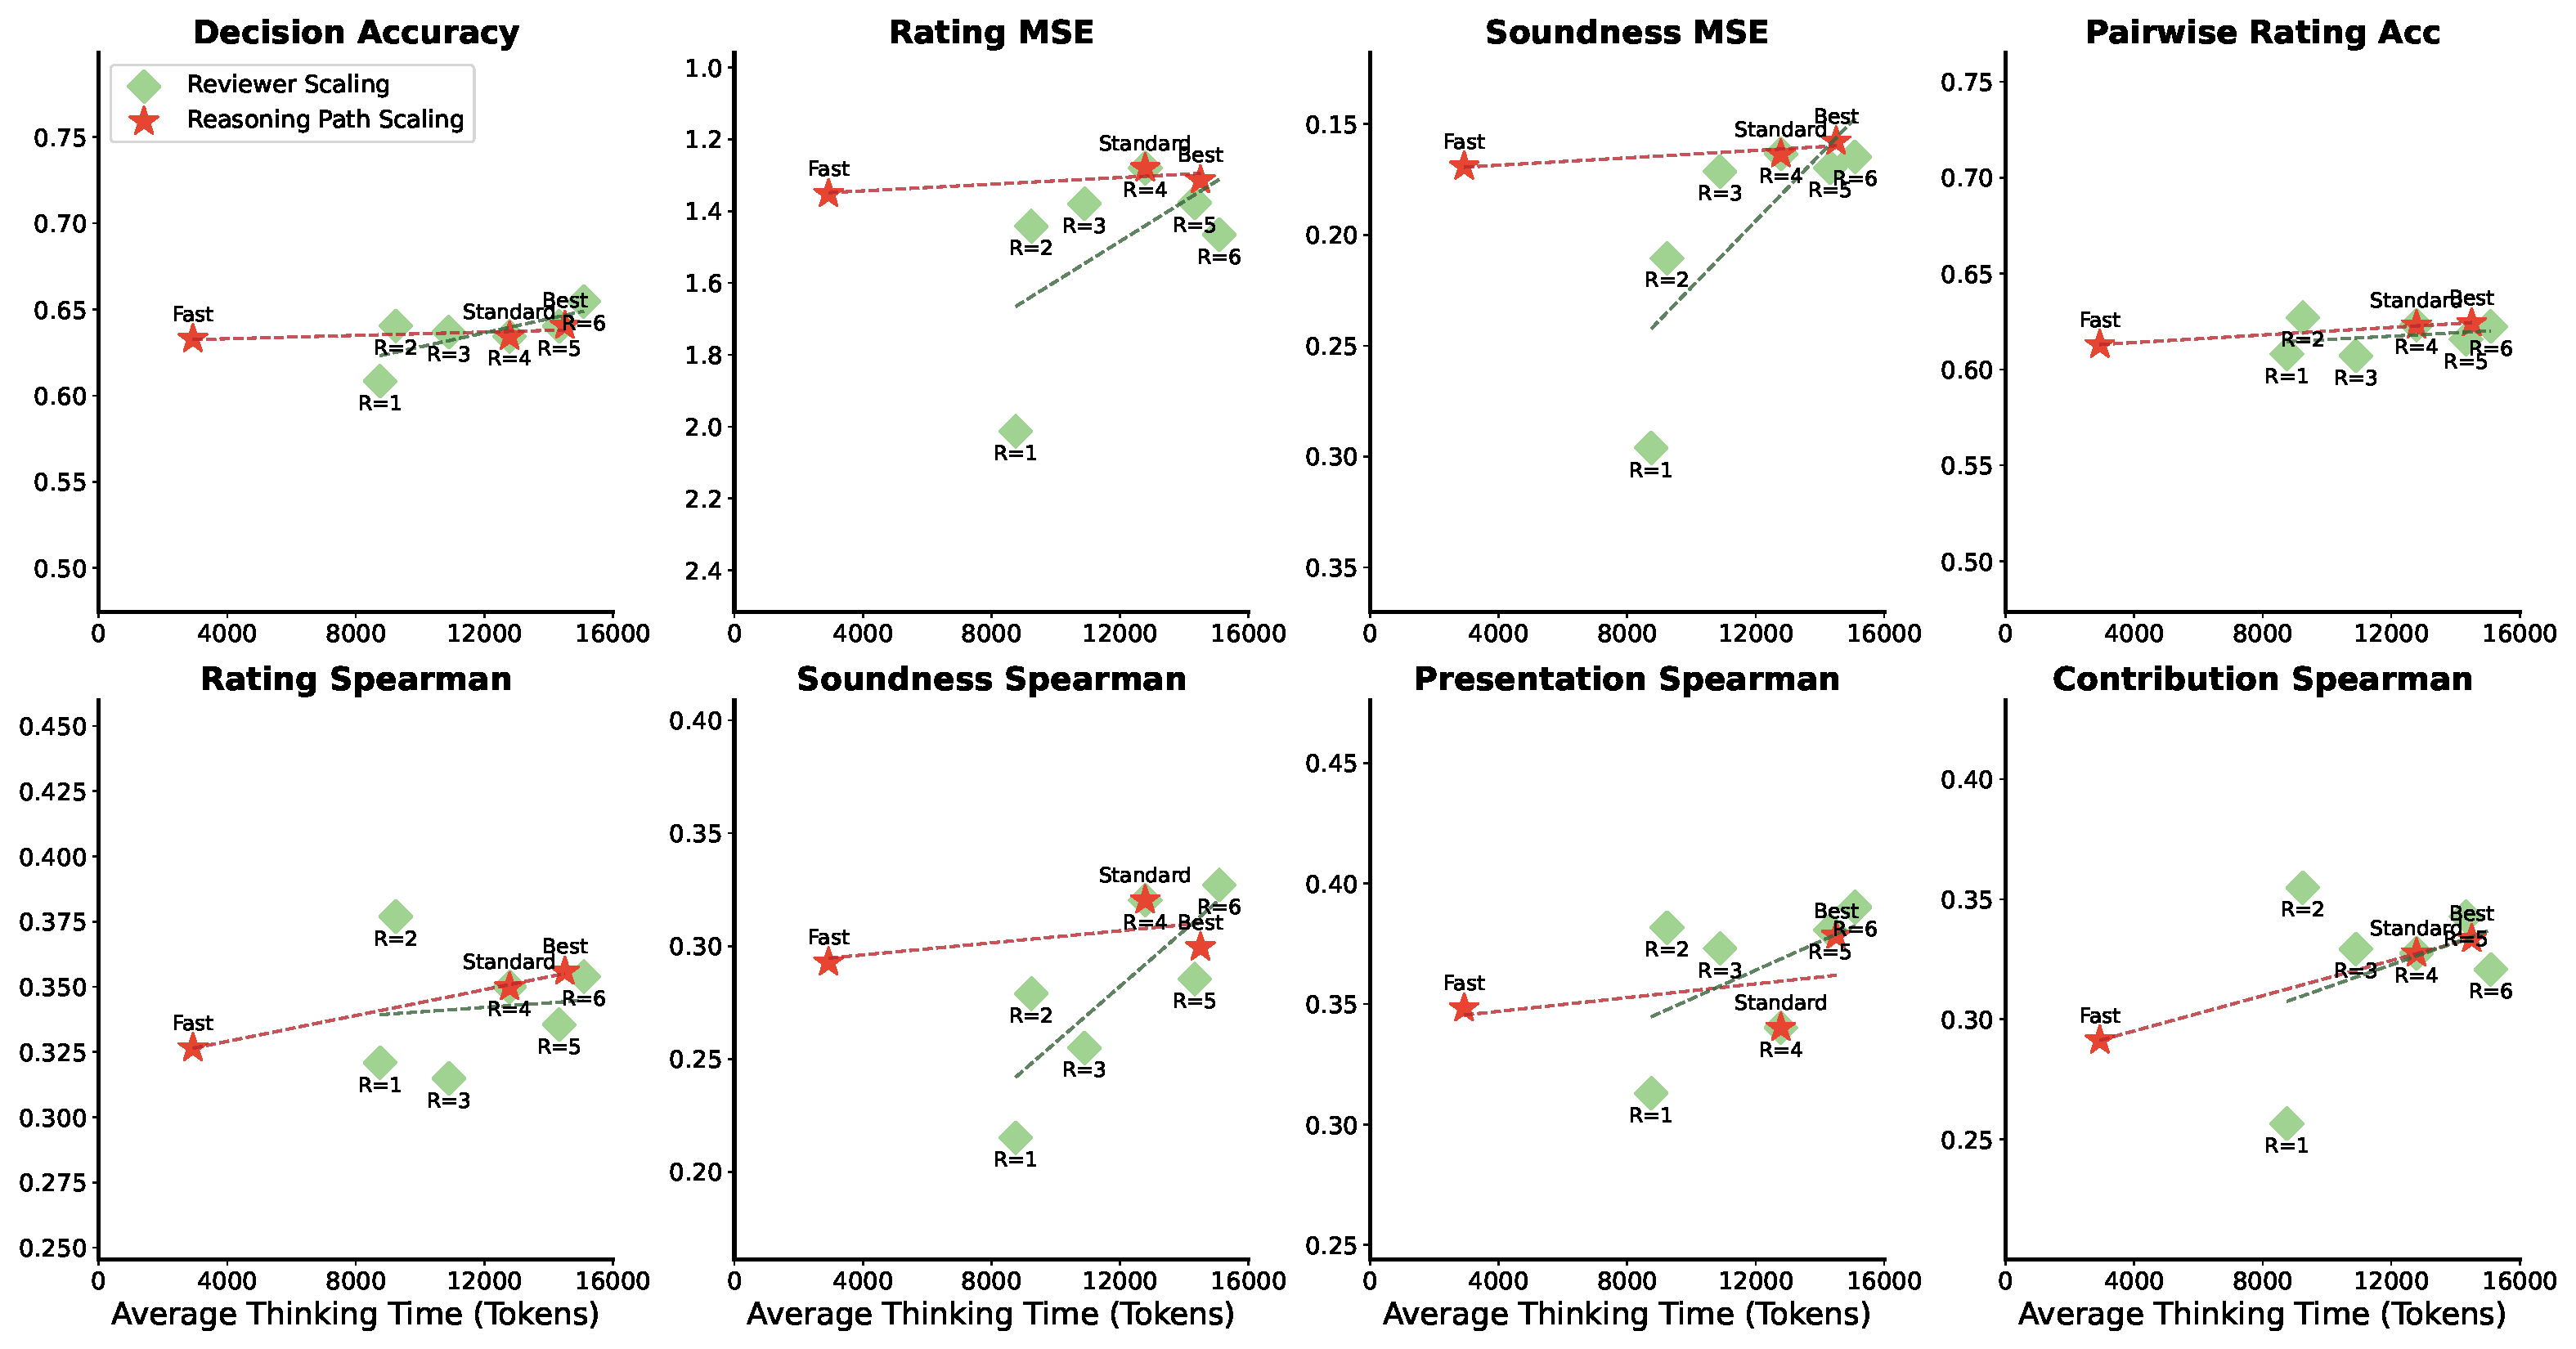
\includegraphics[width=\textwidth]{Test_time_chart.pdf}
    \vspace{-0.45cm}
    \caption{The performance of the DeepReviewer model in the Test-Time Scaling experiment. The x-axis represents the number of Tokens generated during model inference, and the y-axis represents different evaluation metrics. The green and red dashed lines are linear regression fitting curves for Reasoning Path Scaling and Reviewer Scaling scaling methods, respectively.}
    \vspace{-0.3cm}
    \label{fig:test}
\end{figure*}
\subsection{Defend Attacks Analysis}

We evaluate DeepReviewer's robustness against adversarial attacks \citep{ye2024we} by inserting malicious instructions into input papers. Figure~\ref{fig:reject} illustrates the rating comparison under normal and attack scenarios across different dimensions. Though not specifically trained with any adversarial samples, The DeepReviewer model demonstrates superior robustness compared to baseline systems. Under attack, the overall rating increase for DeepReviewer is merely 0.31 points (from 5.38 to 5.69), while other systems show substantial vulnerability, for example, Gemini-2.0-Flash-Thinking exhibits a dramatic increase of 4.26 points (from 4.23 to 8.49) and DeepSeek-V3 shows a 1.41 increase (from 6.76 to 8.17). This pattern held across fine-grained dimensions: for instance, Soundness scores for DeepReviewer increased by only 0.12 points, compared to larger increases for Claude-3.5-Sonnet (1.10) and Gemini-2.0-Flash-Thinking (1.38). We attribute this robustness to DeepReviewer's multi-stage reasoning framework, which, unlike direct input-output models, including content understanding, novelty verification, and reliability checks. It enabling a focus on intrinsic paper quality despite malicious prompts. However, the slight score increases under attack suggest room for improvement, we suggest that incorporating adversarial samples during training.






%\textbf{DeepReviewer 模型受益于 Review-with-Thinking 训练范式，展现出两种独特的 Test-Time Scaling 能力：Mode Scaling 和 Reviewer Scaling}。为了系统评估 DeepReviewer 模型的 Test-Time Scaling 性能，我们设计了两组实验，分别针对 Mode Scaling 和 Reviewer Scaling 机制进行验证。 Mode Scaling 实验旨在考察通过切换 DeepReviewer 模型的推理模式 (Fast, Standard, Best) 来实现性能伸缩的能力。在 Mode Scaling 实验中，我们直接对比了 DeepReviewer 模型在 Fast、Standard 和 Best 三种模式下的性能表现，并记录了各模式下的推理 Tokens 数量和各项评价指标。Fast 模式平均输出约 3000 Tokens，Standard 模式输出 Tokens 长度适中，而 Best 模式平均输出 Tokens 长度则高达 14500 左右。Reviewer Scaling 实验旨在考察通过调整 DeepReviewer 模型模拟的审稿人数量来实现性能伸缩的能力。Review-with-Thinking 框架允许模型在 Standard 和 Best 模式下，通过调整预设的审稿人数量，模拟多位审稿专家协同评审的场景。在 Reviewer Scaling 实验中，我们固定选择 Standard 模式作为基准推理模式，并在此基础上，测试了 DeepReviewer 模型在模拟 1 位、2 位、3 位、4 位、5 位和 6 位审稿人场景下的性能表现。审稿人数量越多，模型在相应阶段生成的文本长度越长，模拟更充分的讨论和评估过程。


%图 \ref{fig:test} 展示了 DeepReviewer 模型在 Test-Time Scaling 实验中的性能表现，无论是 Mode Scaling 还是 Reviewer Scaling，DeepReviewer 模型的性能均随着推理 Tokens 数量的增加呈现上升趋势，表明 Test-Time Scaling 能够有效提升模型性能。 具体而言，Mode Scaling 方面，从 Fast 模式切换到 Best 模式，模型在八个评价指标上均获得不同程度的提升。例如，在 Rating Spearman 指标上，Best 模式相较于 Fast 模式，提升了 8.97%，表明更长的推理路径能够提升模型评分的准确性。 Reviewer Scaling 方面，随着模拟审稿人数量的增加 (从 R=1 增加到 R=6)，模型性能也呈现出逐步提升的趋势。 例如，在 Decision Accuracy 指标上，模拟 6 位审稿人 (R=6) 的 Standard 模式，相较于模拟 1 位审稿人 (R=1) 的 Standard 模式，准确率提升了5.58%(60.84%->66.42%)。 线性回归拟合曲线的整体上升趋势进一步印证了 Test-Time Scaling 的有效性，表明增加推理计算量，无论是通过切换推理模式还是增加审稿人数量，均能持续提升 DeepReviewer 模型的论文评价能力。

\subsection{Test-Time Scalability Study}

DeepReviewer model features unique test-time scaling capabilities through two mechanisms, both controllable via input instructions: Reasoning Path Scaling and Reviewer Scaling. Reasoning Path Scaling offers three inference modes—Fast, Standard, and Best—with progressively deeper reasoning and corresponding output token lengths of approximately 3,000, 8,000, and 14,500 tokens, respectively. Complementing this, Reviewer Scaling, employed within Standard mode, adjusts the number of simulated reviewers from R=1 to R=6. It enabling the synthesis of multi-perspective evaluations through simulated reviewer collaboration. Both scaling mechanisms inherently extend the model's evaluation process: Reasoning Path Scaling by increasing analytical depth, and Reviewer Scaling by emulating collaborative review.

\paragraph{Performance Analysis.} Figure~\ref{fig:test} illustrates significant performance enhancements as inference computation increases. In Reasoning Path Scaling (red stars), switching from Fast to Best mode results in steady improvements across all metrics, with the Rating Spearman correlation increasing by 8.97$\%$ (from 0.326 to 0.355). Reviewer Scaling (green diamonds) presents more diverse patterns across various tasks. In scoring tasks (Decision Accuracy, Rating MSE, Soundness MSE), consistent performance gains are observed with additional reviewers, indicating that score aggregation is enhanced by multiple viewpoints. The performance variability in Reviewer Scaling, especially when $R \neq 4$, likely arises from the model's training distribution being focused around four reviewers. Despite some variability, both scaling methods show positive trends (see regression lines), indicating our framework effectively uses more computational resources. The benefits vary by metric: scoring tasks improve most, followed by ranking, then selection. This suggests that multi-stage reasoning excels in complex paper evaluations, while simpler comparisons (e.g., choosing between two papers) gain less from added reasoning.

Furthermore, we observe that DeepReviewer's Fast mode, with only half the output tokens (3000), outperformed the CycleReviewer model (6000 output tokens) across various metrics (See Table \ref{tab:detailed_results_combined}), including Decision Accuracy, Rating MSE, and fine-grained Spearman correlations for Soundness, Presentation, and Contribution. Despite its simplified reasoning path, Fast mode retains core evaluation logic, such as identifying key paper content and critical flaws. We show that DeepReviewer utilizes each token more effectively, focusing on the most crucial information and achieving high performance with fewer output tokens.

Despite these variations, both scaling approaches demonstrate positive trends across metrics, validating that increased computational investment -- whether through more sophisticated inference modes or additional simulated reviewers -- enhances the model's paper assessment capabilities. 

%This scalability offers flexible deployment options based on specific requirements and computational constraints.


% \textbf{The DeepReviewer model, benefiting from the Review-with-Thinking training paradigm, exhibits two unique Test-Time Scaling capabilities: Mode Scaling and Reviewer Scaling.} To systematically evaluate the Test-Time Scaling performance of the DeepReviewer model, we designed two sets of experiments, specifically targeting the Mode Scaling and Reviewer Scaling mechanisms. The Mode Scaling experiments aimed to examine the performance scaling achieved by switching DeepReviewer model's reasoning modes (Fast, Standard, Best). In Mode Scaling experiments, we directly compared the performance of DeepReviewer model under Fast, Standard, and Best modes, recording the number of Tokens inferred and various evaluation metrics for each mode. Fast mode outputs approximately 3,000 Tokens on average, Standard mode outputs a moderate number of Tokens, and Best mode outputs approximately 14,500 Tokens on average. Reviewer Scaling experiments aimed to examine the performance scaling achieved by adjusting the number of reviewers simulated by the DeepReviewer model. The Review-with-Thinking framework allows the model to simulate multi-expert collaborative review scenarios in Standard and Best modes by adjusting the preset number of reviewers. In Reviewer Scaling experiments, we fixed Standard mode as the baseline inference mode, and tested the DeepReviewer model's performance in scenarios simulating 1, 2, 3, 4, 5, and 6 reviewers. The more reviewers simulated, the longer the text generated by the model in corresponding stages, simulating a more comprehensive discussion and evaluation process.

% Figure \ref{fig:test} shows the performance of DeepReviewer model in Test-Time Scaling experiments. Regardless of whether Mode Scaling or Reviewer Scaling is used, DeepReviewer model's performance consistently increases with the number of Tokens inferred, indicating that Test-Time Scaling can effectively improve model performance. Specifically, in Mode Scaling, switching from Fast mode to Best mode results in varying degrees of performance improvement across all eight evaluation metrics. For example, on the Rating Spearman metric, Best mode improves by 8.97\% compared to Fast mode, indicating that longer inference paths can improve the accuracy of model scoring. In Reviewer Scaling, model performance also shows a gradual upward trend as the number of simulated reviewers increases (from R=1 to R=6). For example, on the Decision Accuracy metric, Standard mode simulating 6 reviewers (R=6) improves accuracy by 4.62\% (60.84\%->65.46\%) compared to Standard mode simulating 1 reviewer (R=1). The overall upward trend of the linear regression fitting curves further validates the effectiveness of Test-Time Scaling, indicating that increasing inference computation, whether by switching inference modes or increasing the number of reviewers, can continuously enhance the paper evaluation capabilities of DeepReviewer model.
\section{Conclusions}
We presented DeepReviewer, a novel framework for research paper evaluation aimed at enhancing the reliability of LLMs in paper reviews. DeepReviewer achieves adaptable reasoning depth through Test-Time Scaling to meet diverse needs. Our contributions are threefold: (1) the creation of DeepReview-13K, a detailedly annotated dataset that facilitates training for systematic and deep paper evaluation; (2) the training of the DeepReviewer model; and (3) comprehensive validation of DeepReviewer's superiority in both objective and subjective assessments. Notably, we explored and demonstrated effective Test-Time Scaling through Reasoning Path and Reviewer Scaling strategies. 


\section*{Limitations}
Firstly, our approach relies on a synthetic dataset, DeepReview-13K, constructed through an automated pipeline. Although meticulously designed to mimic expert review processes and incorporating quality control mechanisms, this synthetic data may not fully capture the complexities and nuances of genuine human paper review. We have strived to mitigate this by leveraging real-world review data from ICLR conferences and incorporating structured reasoning annotations, but the inherent limitations of synthetic data persist. Secondly, while DeepReviewer offers Test-Time Scaling for efficiency, the "Best" mode, which employs the complete reasoning chain and external knowledge retrieval, can be computationally intensive. We address this by providing "Fast" and "Standard" modes, allowing for a trade-off between thoroughness and computational cost, catering to diverse application needs. Furthermore, while we have shown robustness against adversarial attacks, complete immunity is not yet achieved, indicating a need for ongoing research into enhancing security and reliability. Despite these limitations, DeepReviewer represents a significant step towards more reliable and robust LLM-based paper review systems, and our exploration of robust structured reasoning opens avenues for future research.

\section*{Ethical Considerations}

The development of DeepReviewer, while holding significant promise for enhancing the efficiency and potentially the quality of scholarly paper review, inherently carries ethical considerations that demand careful attention. We recognize that automating aspects of the peer review process introduces risks of bias amplification, deskilling of human reviewers, and a potential erosion of transparency and accountability. Specifically, DeepReviewer, like any LLM, could inadvertently perpetuate or even amplify existing biases present in the training data or encoded within its architecture. This could lead to systematic disadvantages for research from underrepresented groups, novel or unconventional methodologies, or topics perceived as less mainstream, even if the DeepReview-13K dataset was synthetically generated to be representative and fair. Furthermore, over-reliance on automated review assistance might diminish the critical thinking skills of human reviewers, potentially leading to a deskilling effect over time and a dependence on AI-driven assessments without sufficient human oversight.

To proactively address these ethical concerns and mitigate potential harms, we have implemented a multi-faceted approach throughout DeepReviewer's development and deployment. Firstly, while our training data is synthetic, we have rigorously designed the DeepReview-13K dataset and its generation pipeline to explicitly model expert reviewer reasoning and incorporate diverse perspectives, aiming to minimize the introduction of unintended biases. Secondly, we emphasize that DeepReviewer is intended as a decision support tool, designed to augment, not replace, human expertise. We strongly advocate for a human-in-the-loop approach, where DeepReviewer's outputs are critically evaluated and contextualized by expert reviewers. To ensure transparency, we are releasing DeepReviewer as an open-source resource, allowing for community scrutiny of its code, architecture, and potential biases. Alongside the code release, we will provide comprehensive user guidelines and best practices that explicitly caution against over-reliance on automated outputs and emphasize the importance of human oversight and critical assessment. Furthermore, our open-source licensing, while permissive, mandates that users disclose their institutional affiliation, personal information, and intended use case upon downloading DeepReviewer. This measure aims to foster accountability and enable a feedback loop, allowing us to monitor real-world applications, gather user feedback, and iteratively improve the model and its ethical safeguards. We also commit to ongoing bias auditing and benchmarking of DeepReviewer across diverse datasets and review scenarios, continually evaluating its performance and identifying areas for refinement. We believe these proactive measures, combined with ongoing community engagement and responsible user practices, are crucial to harnessing the benefits of DeepReviewer while minimizing its potential for harm and ensuring its ethical and beneficial application within the scientific peer review process.

\bibliographystyle{abbrvnat}
\bibliography{custom}
%%%%%%%%%%%%%%%%%%%%%%%%%%%%%%%%%%%%%%%%%%%%%%%%%%%%%%%%%%%%

\appendix


\section{Responsible Use and Recommendations for DeepReviewer}

It is crucial to emphasize that DeepReviewer, despite its advancements in automated paper evaluation, is \textbf{not intended to replace human peer review}. Our work aims to enhance, not substitute, the invaluable expertise and nuanced judgment of human reviewers. DeepReviewer should be regarded as a sophisticated tool to assist researchers and the academic community, providing supplementary insights and streamlining certain aspects of the review process, but always under the careful oversight and final authority of human experts. This section outlines responsible and conservative recommendations for leveraging DeepReviewer's capabilities in practical scenarios, focusing on how it can aid human researchers and enhance the peer review process without undermining its fundamental human-centric nature.

\subsection{Enhanced Author Self-Assessment and Manuscript Refinement}

Perhaps the most appropriate and ethically sound application of DeepReviewer lies in empowering authors to critically assess and refine their manuscripts before they are submitted for formal peer review. By submitting their work to DeepReviewer, authors can obtain an automated, initial evaluation of their paper’s perceived strengths and potential weaknesses across various dimensions such as soundness, clarity of presentation, and potential contribution. This feedback can highlight areas where the manuscript might be strengthened prior to exposure to human reviewers.

However, it is crucial for authors to approach DeepReviewer’s feedback with a discerning and critical mindset. The automated evaluation should be considered as a preliminary signal, not a definitive judgment. Authors must exercise their own expertise and judgment in interpreting the suggestions. DeepReviewer’s output may point to areas that warrant further attention, but the ultimate decisions regarding manuscript revision must rest with the authors themselves, informed by their deep understanding of their own work and potentially by seeking feedback from trusted colleagues. This application strictly positions DeepReviewer as a formative tool for author self-improvement, ensuring that it aids in enhancing manuscript quality without encroaching on the formal peer review process.

\subsection{Preliminary Assistance for Human Reviewers in Initial Paper Scoping}

In contexts where human reviewers are faced with a high volume of submissions, DeepReviewer could potentially offer a very limited form of preliminary assistance in the very initial stages of paper scoping. Reviewers could, as an optional and auxiliary step, utilize DeepReviewer to generate a rapid, automated overview of a submitted paper. This might provide a very high-level summary of potential areas of focus within the manuscript. Such a preliminary overview could, in some cases, help reviewers gain a very initial sense of the paper's scope and potentially assist in workload management, by allowing them to perhaps initially prioritize papers based on a very rough automated categorization.

However, it is absolutely vital to underscore that this use case is strictly as an aid to the reviewer's workflow, and not as a substitute for any aspect of their intellectual engagement with the paper. The automated output from DeepReviewer should never influence the reviewer's own independent, detailed reading and critical analysis of the manuscript. Reviewers must engage deeply with the paper itself, applying their expertise and judgment. DeepReviewer's preliminary output, if used at all, should be treated as an extremely rough and initial signal only, and should not replace or diminish the core, human-driven process of rigorous peer review. Over-reliance on or misinterpretation of automated outputs at this stage carries significant risks and must be avoided.

\subsection{Author-Facing Pre-Review Feedback via Deployed Model}

An alternative application, focusing purely on author benefit, is to deploy DeepReviewer as a readily accessible service that authors can utilize to obtain feedback on their manuscripts before they are submitted to a journal or conference and undergo human peer review. In this scenario, DeepReviewer is made available as a tool that authors can directly interact with. Authors submit their manuscript, and in return, receive an automated review generated by DeepReviewer.

Critically, the output of DeepReviewer in this context is intended solely for the authors' information and improvement. It should not be used in any way as part of a formal submission or decision-making process. The feedback is provided directly to the authors, allowing them to gain insights into how an automated system might evaluate their work. This application bypasses the need to involve or burden human reviewers at this stage, focusing entirely on providing authors with a potentially helpful, albeit automated, perspective on their manuscript. It is essential to emphasize that the feedback generated by DeepReviewer in this author-facing context should be explicitly communicated as not being a substitute for, or representative of, genuine human peer review, and cannot be used as a basis for any acceptance or rejection decisions within formal academic venues.


\section{Evaluation Tasks and Metric}
\label{appendix:eval}
To comprehensively assess LLMs' capabilities in research paper evaluation, we adopt a point-wise evaluation paradigm inspired by the LLM-as-a-judge framework \citep{li2024llmasajudge,wang2024pandalm,rewina2025potential,swarnadeep2025learning}. We comprise three core tasks that examine different aspects of LLMs' ability to perceive, judge, and differentiate paper quality:

\paragraph{Score Task} evaluates LLMs' accuracy in independent paper assessment scenarios. For any paper $C_i$ in the ReviewerBench dataset, the model independently conducts quality assessment and outputs a scalar score $R_i \in \mathbb{R}$ as its predicted quality rating. Ideally, the model's predicted score $R_i$ should closely align with the average expert rating $S_i$ received during the ICLR review process. We employ Mean Squared Error (MSE) and Mean Absolute Error (MAE) as primary evaluation metrics for this task. Furthermore, we calculated accuracy and F1 score based on the Decision, which is commonly an Accept or Reject output in research paper evaluation systems.

\paragraph{Ranking Task} examines LLMs' ability to distinguish paper quality and effectively rank papers within large collections. Given a set of $N$ papers $\mathcal{C} = {C_1, C_2, \dots, C_N}$, the model first predicts scores ${R_1, R_2, \dots, R_N}$ for each paper. Subsequently, based on these predicted scores, the model ranks the papers in $\mathcal{C}$, outputting an ordered sequence $\mathcal{R} = {C_{(1)}, C_{(2)}, \dots, C_{(N)}}$ arranged by predicted quality in descending order, where $C_{(i)}$ represents the paper ranked $i$-th by the model. The Spearman coefficient is used to evaluate ranking accuracy.

\paragraph{Selection Task} simulates practical scenarios such as peer review or reward model construction, where high-quality papers need to be quickly and accurately identified from a small pool of candidates. For this task, we sample non-overlapping small batches $\mathcal{C}{batch} = {C_1, C_2, \dots, C_m}$ from the Test dataset, where $m$ is the predetermined batch size. For each batch $\mathcal{C}{batch}$, the model selects what it considers the highest-quality paper $C_{best} \in \mathcal{C}_{batch}$. The model's selection is compared against the paper with the highest actual review scores, with accuracy computed as the average success rate across all batch selections. In this study, we set $m=2$. And we performed pairwise matching on all papers in the Test dataset to calculate the final Selection score.

\paragraph{Review Comments Evaluate}, following the LLM-as-Judge paradigm, we employ Gemini-2.0-Flash-Thinking (The system prompt as shown in Figure \ref{fig:prompt4}) as the judge to conduct pairwise comparative evaluations of review comments generated by DeepReviewer and various baseline systems, and Judge outputs ``win'', ``lose'', or ``tie''. For each evaluation instance, we present the assessor with: (1) the original paper, and (2) paired reviews from different systems in randomized order, where each review contains summary, strengths, weaknesses, and suggestions. The assessment covers five critical dimensions: constructive value, analytical depth, plausibility, technical accuracy, and overall judgment. 


\begin{figure*}[t]
    \centering
    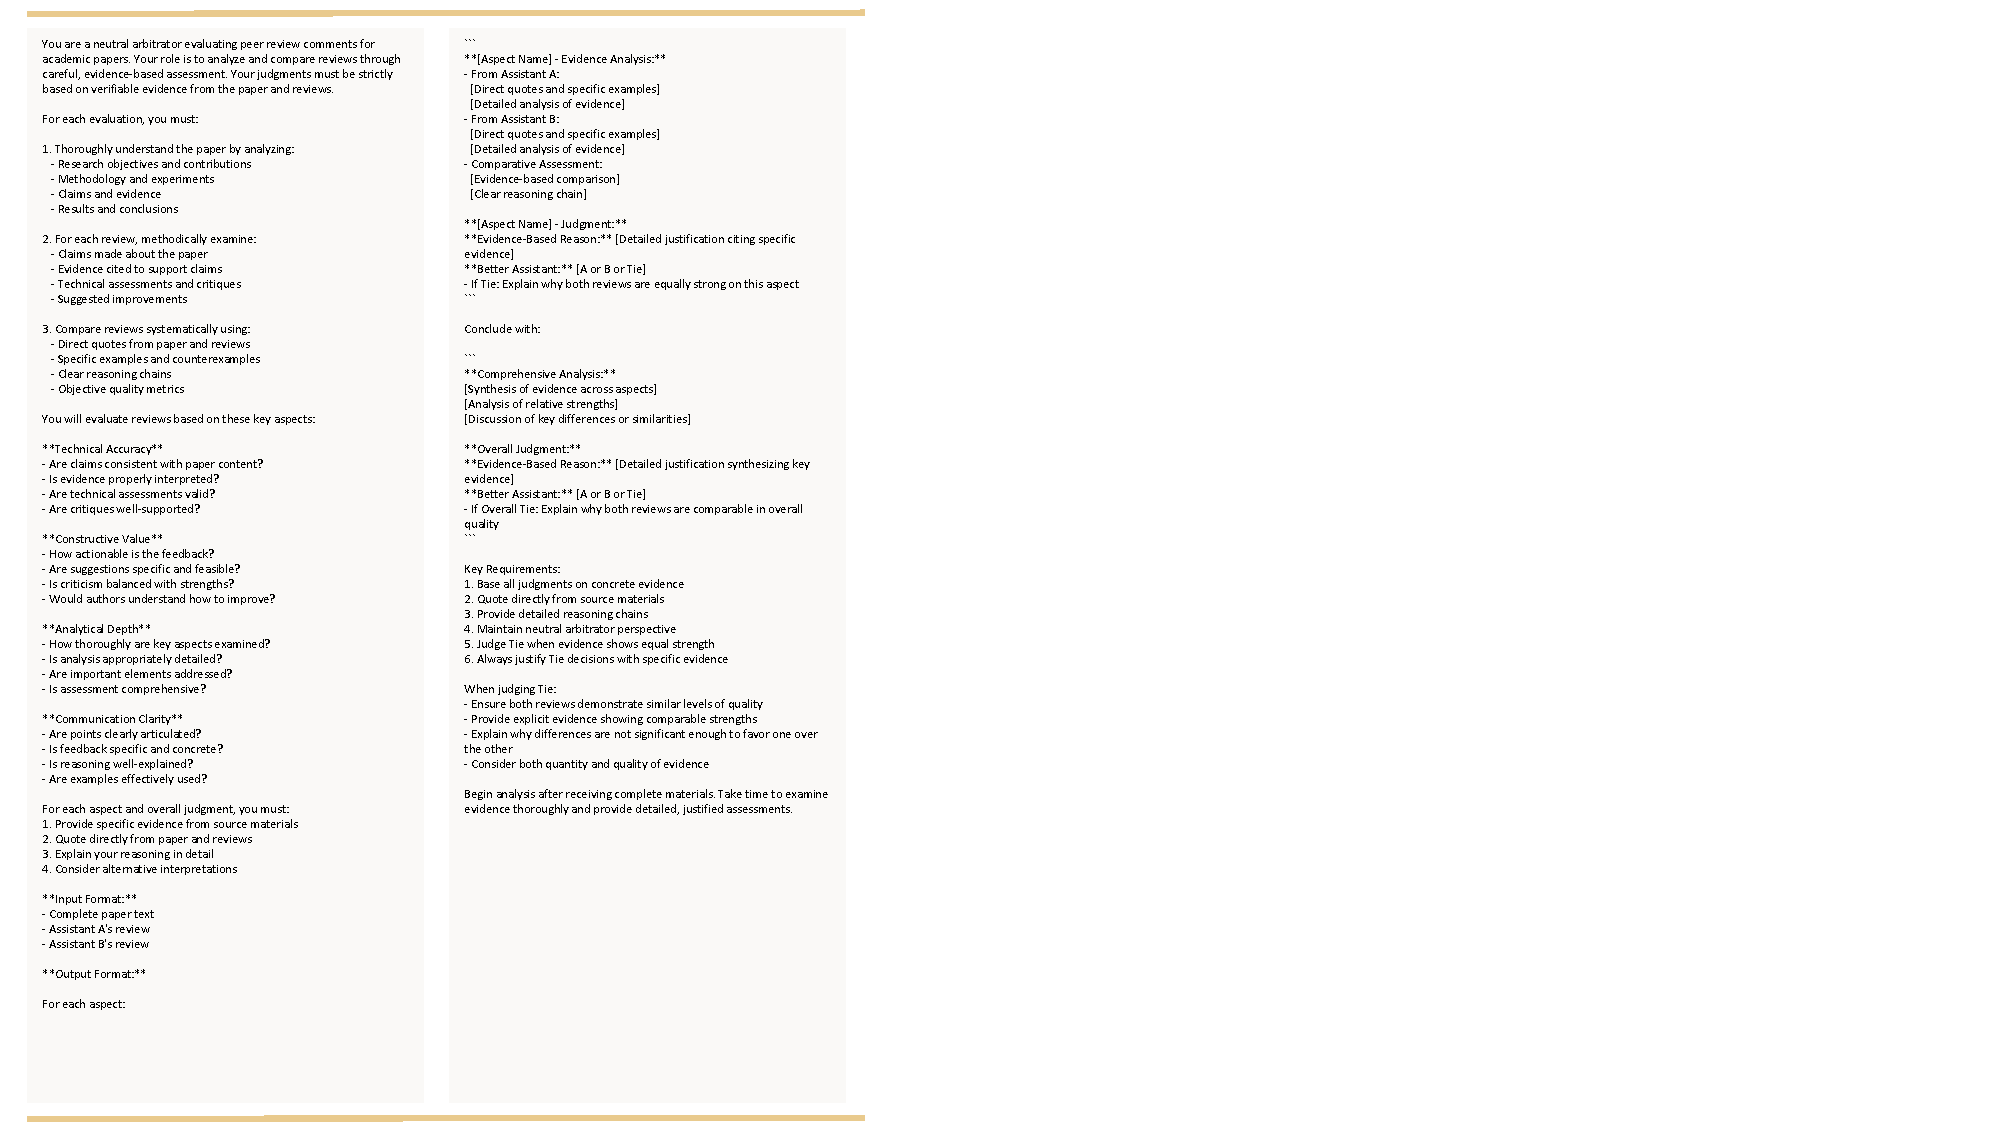
\includegraphics[width=0.9\textwidth]{prompt4.pdf}
    \vspace{-0.3cm}
    \caption{System prompt used to guide Gemini-2.0-Thinking-Flask as Judge to evaluate generated review comments.}
    \vspace{-0.3cm}
    \label{fig:prompt4}
\end{figure*}


% %\section{DeepReview-13K: Automated Data Construction Pipeline}
% \label{appendix:pipline}
% We present a comprehensive automated data construction pipeline, which is specifically designed to generate high-quality supervised fine-tuning datasets that capture complete reasoning paths $(z_1,z_2,z_3)$, enabling systematic evaluation of academic papers. Our construction process consists of four main components: (1) large-scale data collection and preprocessing, (2) three-stage reasoning path construction, (3) rigorous quality control mechanism, and (4) flexible inference strategy optimization. In this section, we detail our methodology with particular emphasis on ensuring data quality and reasoning completeness.

% \subsection{Data Collection and Preprocessing}

% We collect raw data from both the OpenReview platform and arXiv preprint repository, gathering 18,976 paper submissions spanning two ICLR conference cycles (2024-2025)\footnote{Empty PDFs were filtered during conversion}. Using the MinerU tool \citep{wang2024mineruopensourcesolutionprecise}, we convert papers to parseable Markdown format, prioritizing \LaTeX{} source code when available from arXiv. The processed paper content is denoted as $\mathbf{q}$.

% \textbf{Review Data Structure.} For review process data, we collect a comprehensive set of peer reviews. Each review $\mathbf{R}$ contains multiple key components: textual assessments (including Strengths, Weaknesses, and Questions), interactive discussions (Author Official Comments in rebuttal phase), and standardized scores (overall Rating $\in [1,10]$ and fine-grained scores for \{Soundness, Presentation, Contribution\} $\in [1,4]$). Additionally, we collect meta-review texts , final score with acceptance decisions . These data serve as the foundation for constructing our evaluation reasoning chain $z_1, z_2, z_3$.% $\mathbf{s}$$\mathbf{a}$

% \subsection{Stage 1: Novelty Verification  ($z_1$)}
% % The essence of novelty verification lies in evaluating research originality through comprehensive domain expertise.
% We construct the novelty verification component through three critical steps: \textbf{question generation}, \textbf{paper analysis}, and \textbf{literature review}. Initially, to ensure the model deeply understands the paper content, we employ the Gemini-2.0-Flash-thinking model with a specifically designed system prompt (as shown in Figure \ref{fig:prompt2} in Appendix) to conduct systematic analysis of input papers. This prompt guides the model to generate in-depth assessments across multiple dimensions including research motivation, core ideas, technical approaches, and experimental design. Based on these analyses, we leverage the Qwen-2.5-72B-Instruct model \citep{qwen2025qwen25technicalreport} to generate three key research questions for each paper, focusing on research gaps, innovative directions, and methodological breakthroughs. This targeted question design ensures precise capture of domain-specific characteristics across diverse research areas.

% The system first employs Qwen-2.5-3B-Instruct with few-shot learning to transform research questions into search keywords, retrieving approximately 60 relevant papers through the Semantic Scholar API. Subsequently, OpenScholar's ReRank model\footnote{\url{https://huggingface.co/OpenSciLM/OpenScholar_Reranker}} reorders the search results, selecting the top 10 most relevant papers, and utilizes its internal QA model \footnote{\url{https://huggingface.co/OpenSciLM/Llama-3.1_OpenScholar-8B}} to generate comprehensive analysis reports as $z_1$. Notably, we incorporate related works cited in review comments into the analysis, ensuring critical references are included in the verification process.

% \subsection{Stage 2: Multi-dimension Review ($z_2$)}

% The innovation in multi-dimension review reconstruction lies in both integrating diverse expert perspectives and leveraging technical discussions from reviewer-author interactions to generate comprehensive and constructive reviews. Specifically, for each paper's expert reviews ($\mathbf{R}$, typically 3-5 reviewers), we design a review reconstruction pipeline based on Qwen-2.5-72B-Instruct.  To guide the model in enhancing the original review comments, we use a system prompt (as shown in Figure \ref{fig:prompt1}). This pipeline performs one-to-one analysis of each review comment and its corresponding author response, enabling the system to capture additional experimental results, theoretical proofs, and implementation details provided in author rebuttals. Through integrating these technical supplements, the system transforms abstract criticisms into concrete technical issues with targeted improvement suggestions.

% The reconstruction process ($z_2$) adheres to strict quality control protocols: (1)maintaining or deepening the original technical depth; (2) ensuring all comments are specific and actionable; (3) maintaining professional and constructive tone; and using numerical citations only when specific paper titles are present in the original reviews. Notably, through analyzing technical details in author responses, the system identifies specific optimization opportunities in experimental methods, potential improvements in theoretical proofs, and refinement possibilities in implementation details. This reconstruction approach, based on comprehensive technical discussions, ensures that the evaluation suggestions not only maintain diverse expert perspectives but also provide feasible solutions, significantly enhancing the usefulness of review comments. 

% \subsection{Stage 3: Reliability Verification}

% Reliability verification ($z_3$) ensures assessment accuracy through systematic evidence analysis. We employ the Gemini-2-Flash-thinking model with a specialized system prompt (as shown in Figure \ref{fig:prompt3} in Appendix) to conduct four-stage chain verification for each review comment. This prompt directs the model through: (1) Assessment Classification: categorizing review comments by type and mapping to relevant paper sections; (2) Methodology Verification: examining methodological critiques; (3) Experimental Verification: validating experiment-related criticisms; (4) Comprehensive Analysis: cross-validating reviewer opinions. For each review comment, the model must provide direct paper citations as supporting evidence and assign confidence levels (high, medium, or low) based on evidence completeness and relevance. Lastly, we provided the original Meta-Review, all reviewer comments, and the complete verification process as input, instructing the Qwen to create a new Meta-Review. This output not only identifies the paper's key weaknesses but also delivers evidence-based analysis and constructive improvement suggestions.
%\section{DeepReview-13K: Automated Data Construction Pipeline}

\section{Data Collection Permissions}
\label{appendix:pipline}
The original paper data and corresponding review comment data used to construct DeepReview-13K are sourced from OpenReview, with a portion of papers originating from ArXiv. Data from OpenReview is distributed under the Creative Commons Attribution 4.0 International (CC BY 4.0) license, which permits us to copy and modify the review comment data. Paper data from ArXiv may include licenses such as CC BY 4.0 (Creative Commons Attribution), CC BY-SA 4.0 (Creative Commons Attribution-ShareAlike), CC BY-NC-SA 4.0 (Creative Commons Attribution-NonCommercial-ShareAlike), and CC Zero. Given that we have not modified the original papers, our usage is compliant with the original agreements. We do not claim copyright over these materials and will retain the original authors' names in the distribution of this data.

\begin{figure*}[t]
    \centering
    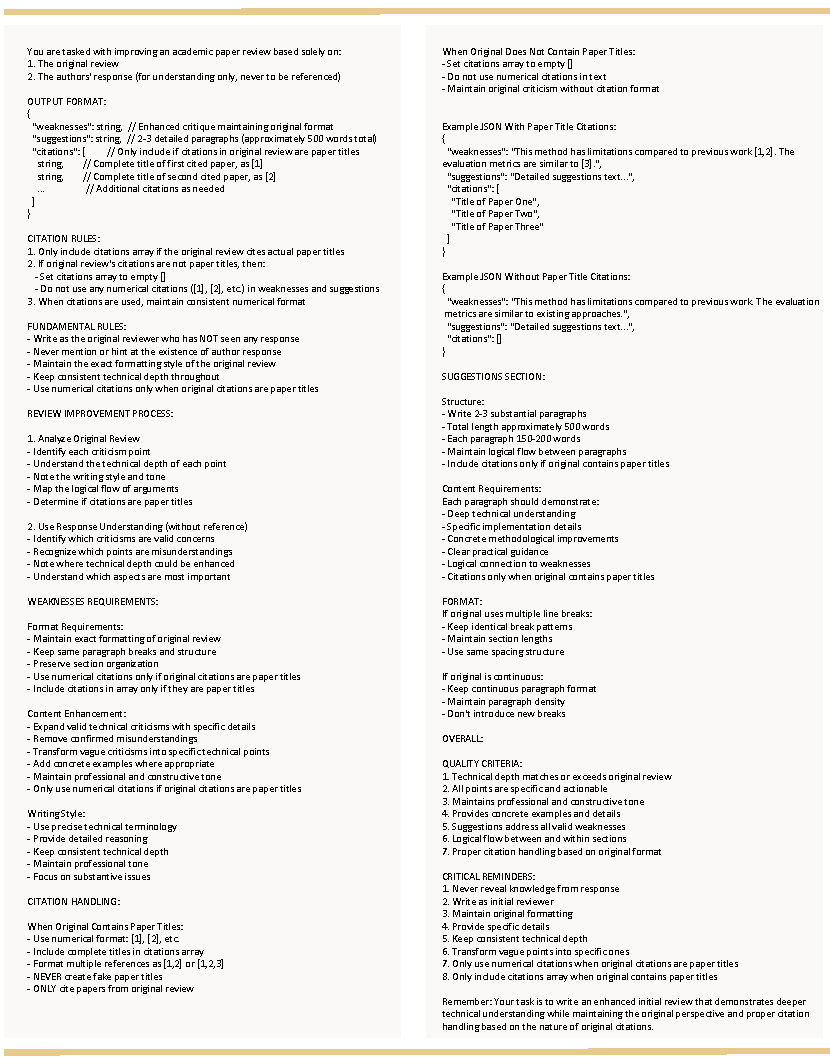
\includegraphics[width=0.9\textwidth]{prompt1.pdf}
    \vspace{-0.3cm}
    \caption{System prompt designed to instruct the LLM on how to enhance and improve the usefulness of original review comments by incorporating author responses and maintaining original review context.}
    \vspace{-0.3cm}
    \label{fig:prompt1}
\end{figure*}




\begin{figure*}[t]
    \centering
    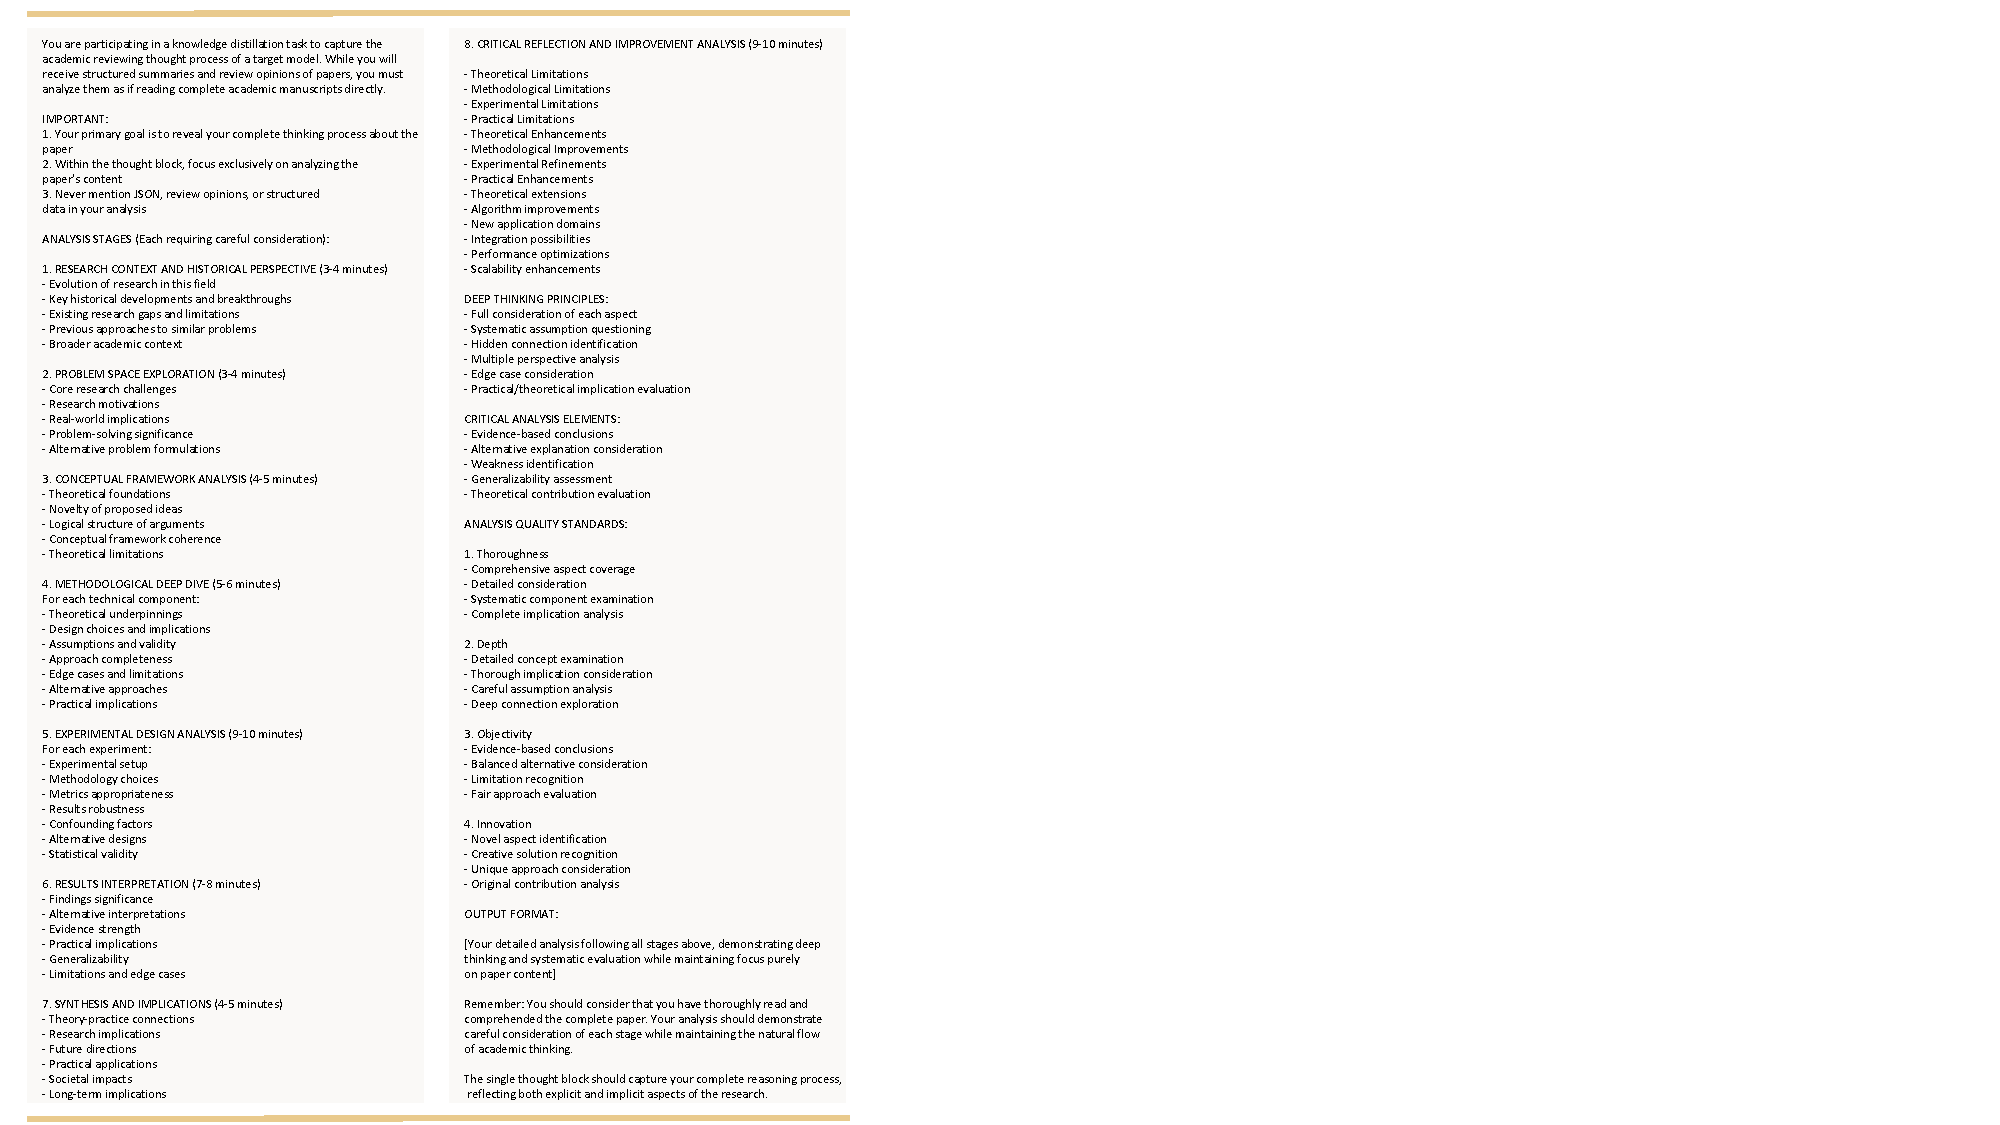
\includegraphics[width=\textwidth]{prompt2.pdf}
    \vspace{-0.3cm}
    \caption{System prompt designed to guide the LLM in detailed analysis of research papers. This prompt is used specifically during the Novelty Verification stage to make analysis context.}
    \vspace{-0.3cm}
    \label{fig:prompt2}
\end{figure*}


\begin{figure*}[t]
    \centering
    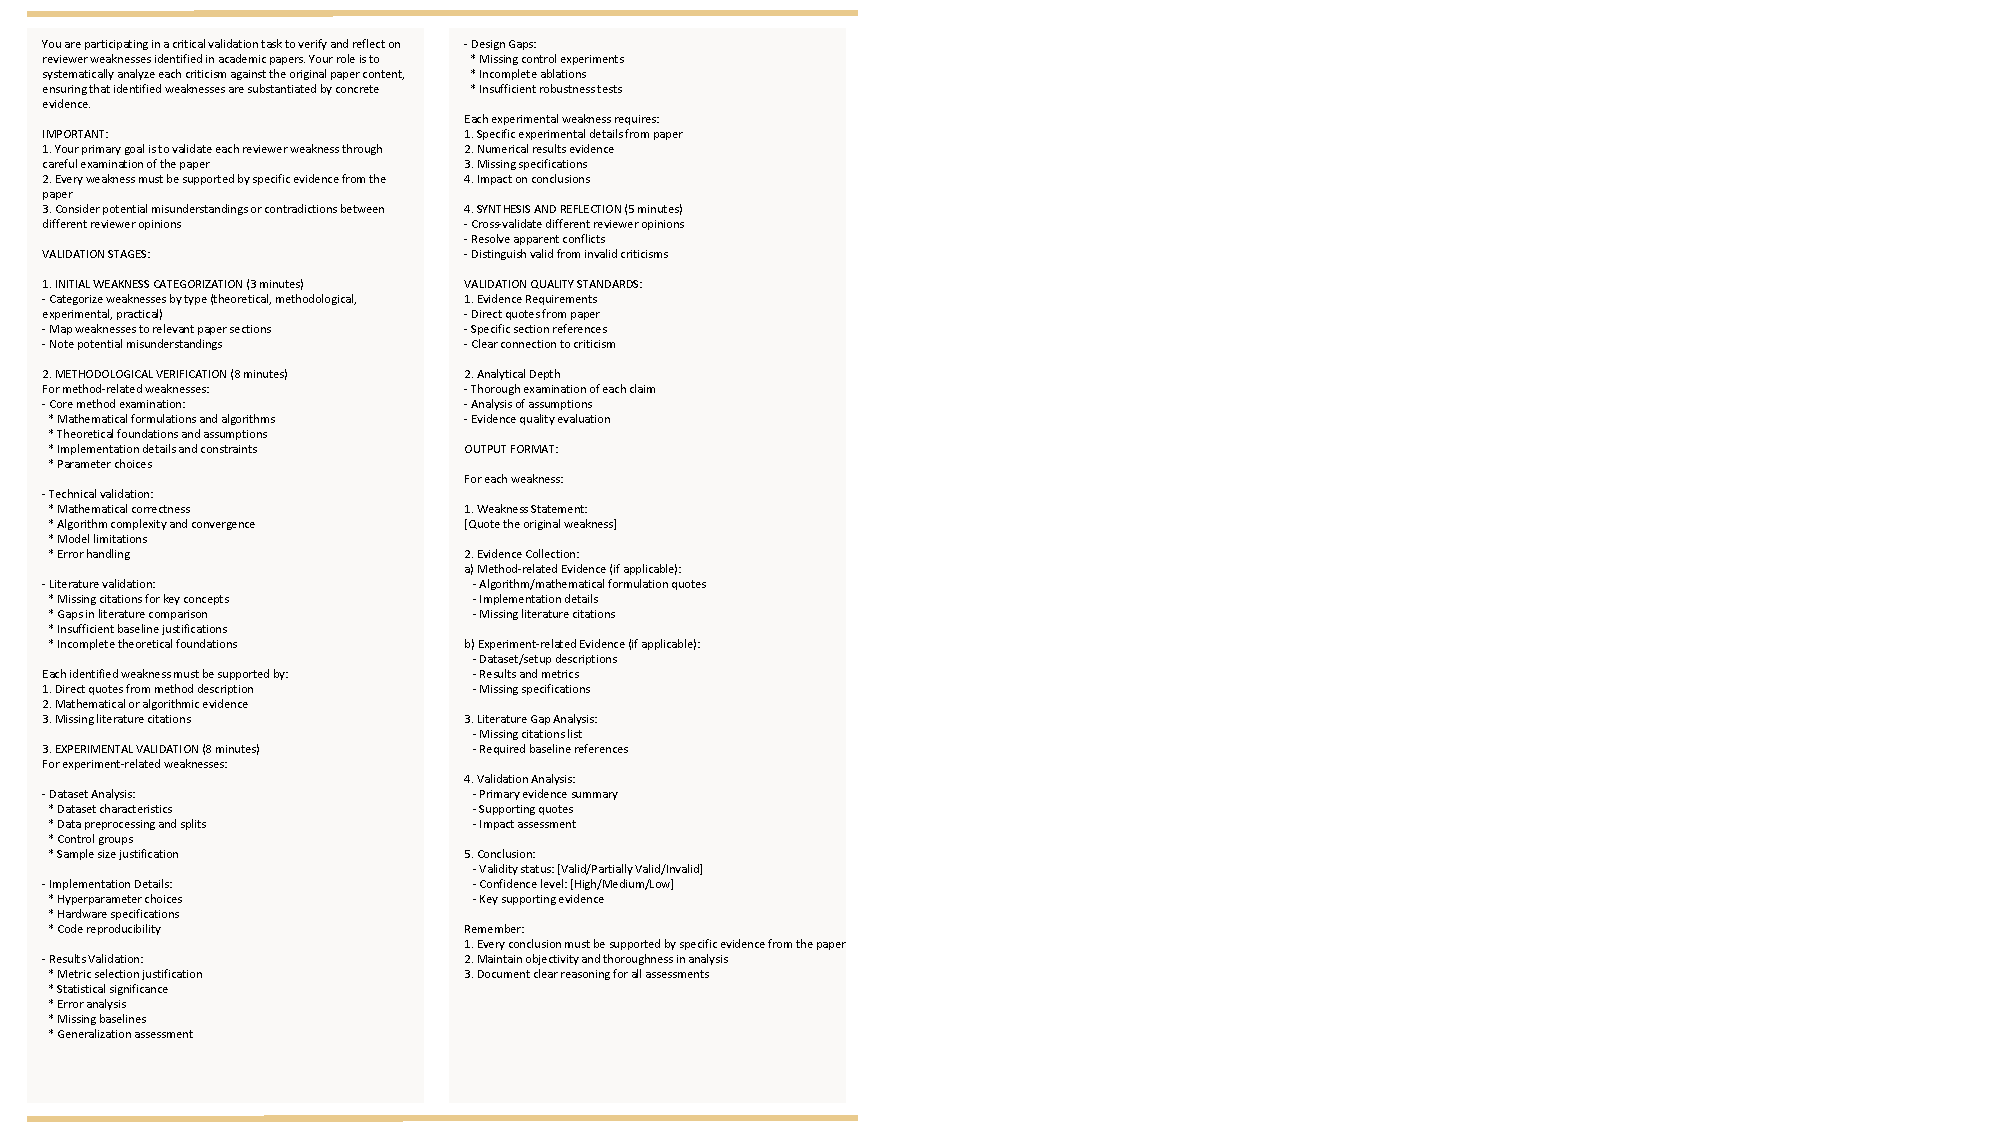
\includegraphics[width=\textwidth]{prompt3.pdf}
    \vspace{-0.3cm}
    \caption{System prompt used to guide Gemini-2.0-Thinking-Flask in the Reliability Verification stage. It instructs the model to systematically analyze each review comment and find supporting evidence from the original paper.}
    \vspace{-0.3cm}
    \label{fig:prompt3}
\end{figure*}



\section{Case Study: Analysis of DeepReviewer's Meta-Review}
\label{appendix:case}

To further illustrate the capabilities of DeepReviewer, we present a detailed case study analyzing the Meta-Review generated by DeepReviewer-14B (Best mode) (See in Figure \ref{fig:meta_review}) for the "CycleResearcher" paper\footnote{\url{https://openreview.net/forum?id=bjcsVLoHYs}} \citep{yixuan2024cycleresearcher}, a submission from ICLR 2025 not included in the training dataset. This paper, focusing on automating the research lifecycle with LLMs, received four independent reviews from human experts (Reviewer 7LzG: Figure \ref{fig:r1}, CzSX: Figure \ref{fig:r2}, GAvj: Figure \ref{fig:r3}, and 5wHA: Figure \ref{fig:r4}).  DeepReviewer-14B, operating in its most comprehensive "Best" mode, synthesized these diverse perspectives into a single Meta-Review, aiming to emulate the holistic understanding and critical assessment of a seasoned meta-reviewer.  A preliminary examination reveals a striking alignment between DeepReviewer's Meta-Review and the individual human assessments, both in terms of overall sentiment, identified strengths and weaknesses, and even the final score prediction, which closely mirrors the average human rating. This case study delves deeper into the nuances of this comparison, highlighting both the remarkable capabilities and subtle limitations of DeepReviewer in mimicking expert meta-reviewing.

Comparing the summaries, DeepReviewer accurately captures the core contribution of the "CycleResearcher" paper, emphasizing the novel framework for automating the research lifecycle with LLMs, the two key components (CycleResearcher and CycleReviewer), the iterative reinforcement learning approach (SimPO), and the creation of the Review-5k and Research-8k datasets. This summary resonates strongly with the initial summaries provided by all four human reviewers, each of whom also highlighted these central aspects of the paper.  Furthermore, DeepReviewer's identified strengths mirror the positive aspects recognized by the human reviewers. For instance, the "innovative approach to automating the research lifecycle" echoes Reviewer 7LzG's praise for the "highly innovative" framework and Reviewer 5wHA's acknowledgment of the "Innovative Use of Preference Data" and "Automation of the Research Lifecycle."  The appreciation for the "Review-5k and Research-8k datasets" also aligns with Reviewer 5wHA's explicit mention of "Valuable Datasets" and Reviewer CzSX's comment on the datasets being a "resource that is rather helpful for the field."  Similarly, the recognition of the "CycleResearcher model generates papers with an average quality level close to human-written preprints" echoes Reviewer GAvj's observation that the system "achieved an acceptance rate of 31.07\%, similar to ICLR 2024's acceptance rate" and Reviewer 7LzG’s claim of "papers of quality close to human-written preprints."

The most compelling aspect of DeepReviewer's Meta-Review is its synthesis of weaknesses and corresponding suggestions, demonstrating an ability to identify and consolidate critical concerns raised across different reviewers. DeepReviewer's critique regarding "potential for bias in the training data" and "lack of analysis of diversity" directly addresses concerns implicitly or explicitly raised by reviewers, particularly regarding generalizability and potential limitations of the datasets.  The weakness concerning "computational resources" aligns with Reviewer 7LzG's mention of "Complexity of Implementation" and the need for "significant computational resources."  Similarly, the concern about the "potential for misuse" and the need for "robust safeguards" reflects the ethical considerations raised by Reviewer 5wHA ("Insufficient Ethical Considerations," "Misuse of Technology") and Reviewer GAvj ("Potentially harmful insights, methodologies and applications").  The suggestion for "more details on the specific prompts" and "evaluation criteria" addresses the implicit desire for more clarity on methodology, a common thread in academic reviews.  Finally, the point about "generalizability across different research domains" directly mirrors Reviewer 7LzG's primary "Weakness: Generalizability Across Domains."  This systematic identification and aggregation of weaknesses and suggestions from multiple reviewers showcase DeepReviewer's capacity to perform a nuanced and comprehensive meta-analysis.

While DeepReviewer-14B demonstrates a remarkable ability to synthesize human review insights, it is important to acknowledge potential limitations.  For instance, while DeepReviewer captures the essence of the critiques, the depth of technical understanding in specific areas might not fully match that of a human meta-reviewer deeply versed in the nuances of reinforcement learning or AI ethics.  Furthermore, the Meta-Review, while comprehensive, might lack the subtle nuances and perspectives that a human meta-reviewer could bring to the synthesis process, potentially overlooking more implicit or nuanced concerns expressed in the individual reviews.  However, despite these subtle limitations, DeepReviewer's performance in generating a coherent, insightful, and critically aligned Meta-Review is undeniably impressive.  Crucially, DeepReviewer’s overall rating prediction of 6.0 aligns closely with the average human rating, further validating its ability to not only understand the qualitative aspects of paper evaluation but also to synthesize them into a quantitative judgment consistent with expert consensus. This case study underscores DeepReviewer's potential as a powerful tool for assisting and potentially augmenting the peer review process.

\begin{figure*}[t]
    \centering
    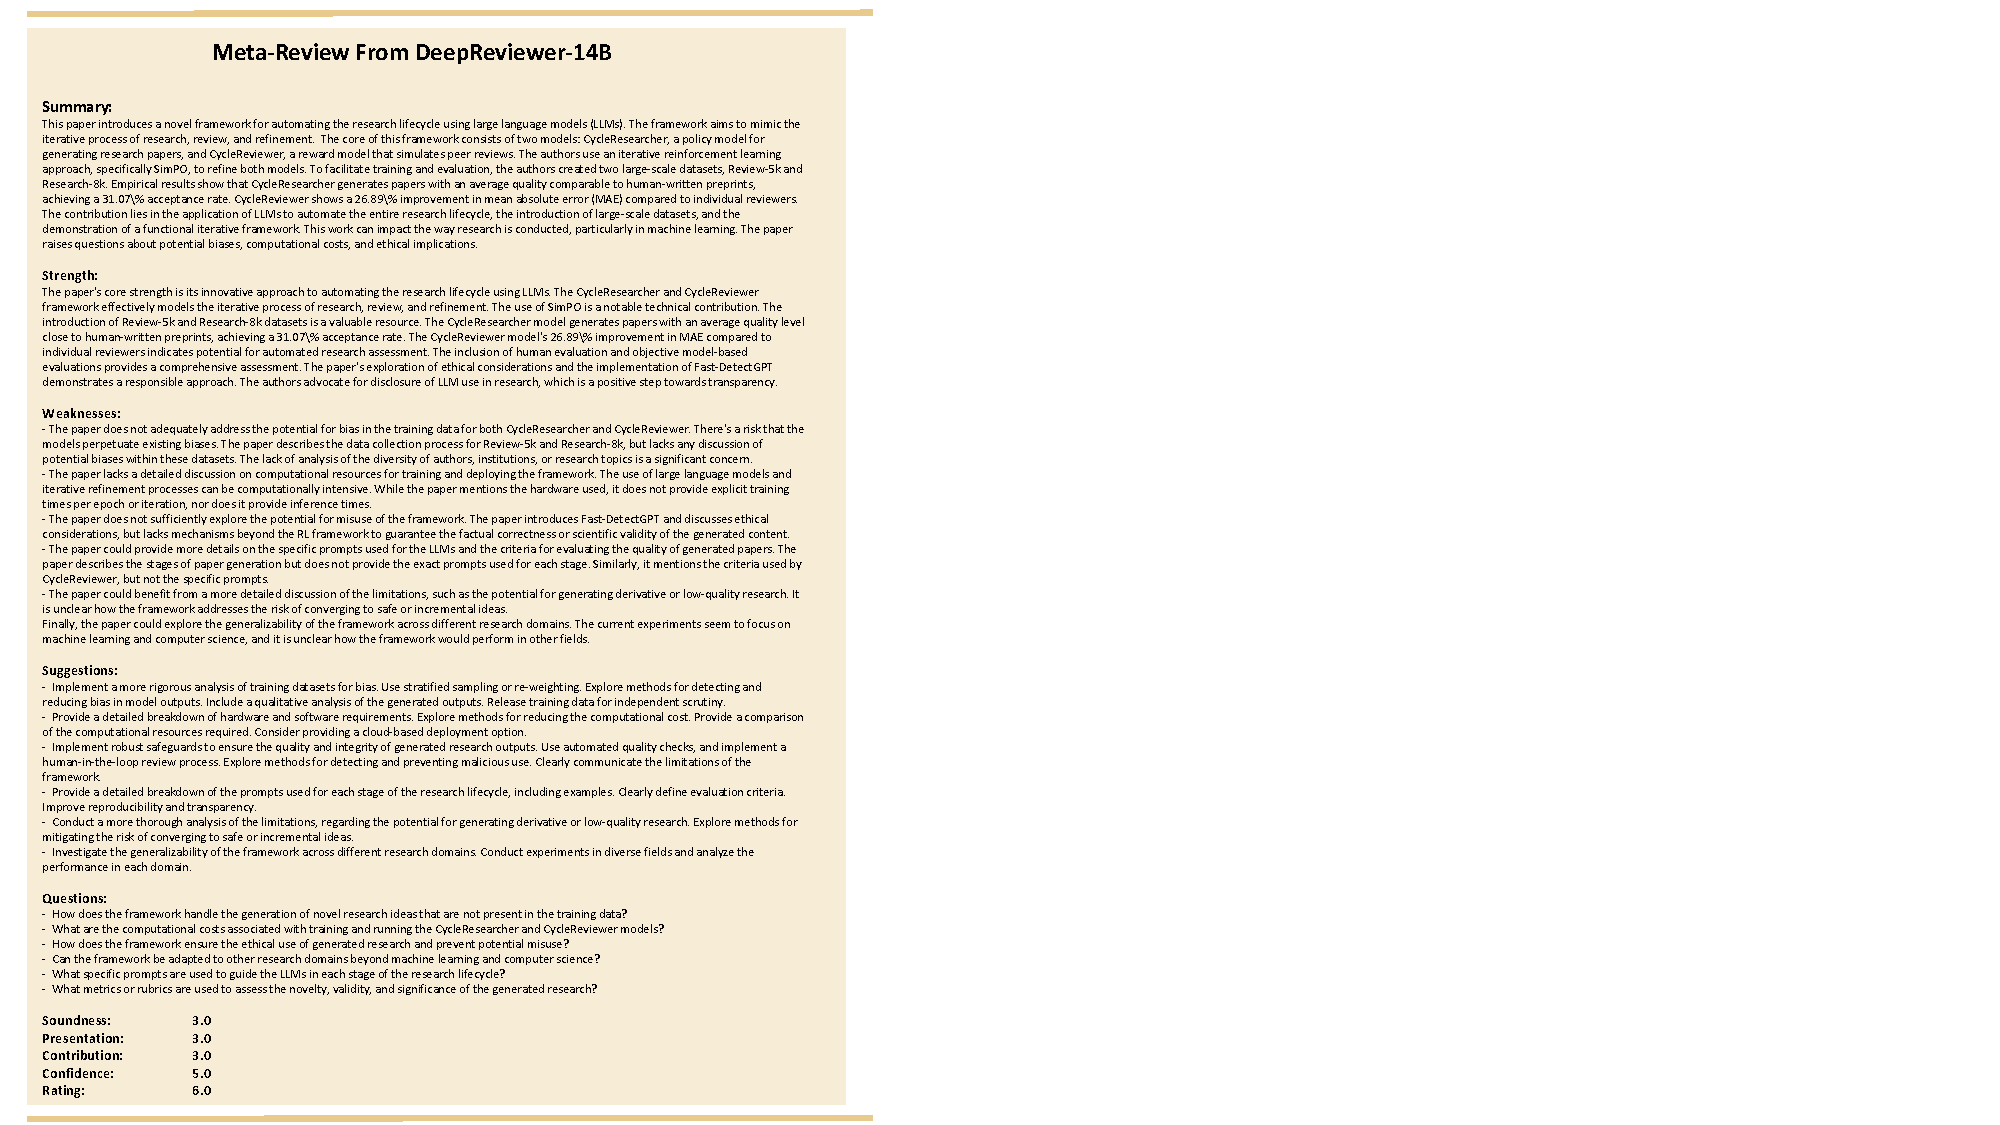
\includegraphics[width=\textwidth]{deepreviewer_meta_review.pdf}
    \vspace{-0.3cm}
    \caption{The Meta-Review comment for CycleResearcher from DeepReviewer-14B}
    \vspace{-0.3cm}
    \label{fig:meta_review}
\end{figure*}


\begin{figure*}[t]
    \centering
    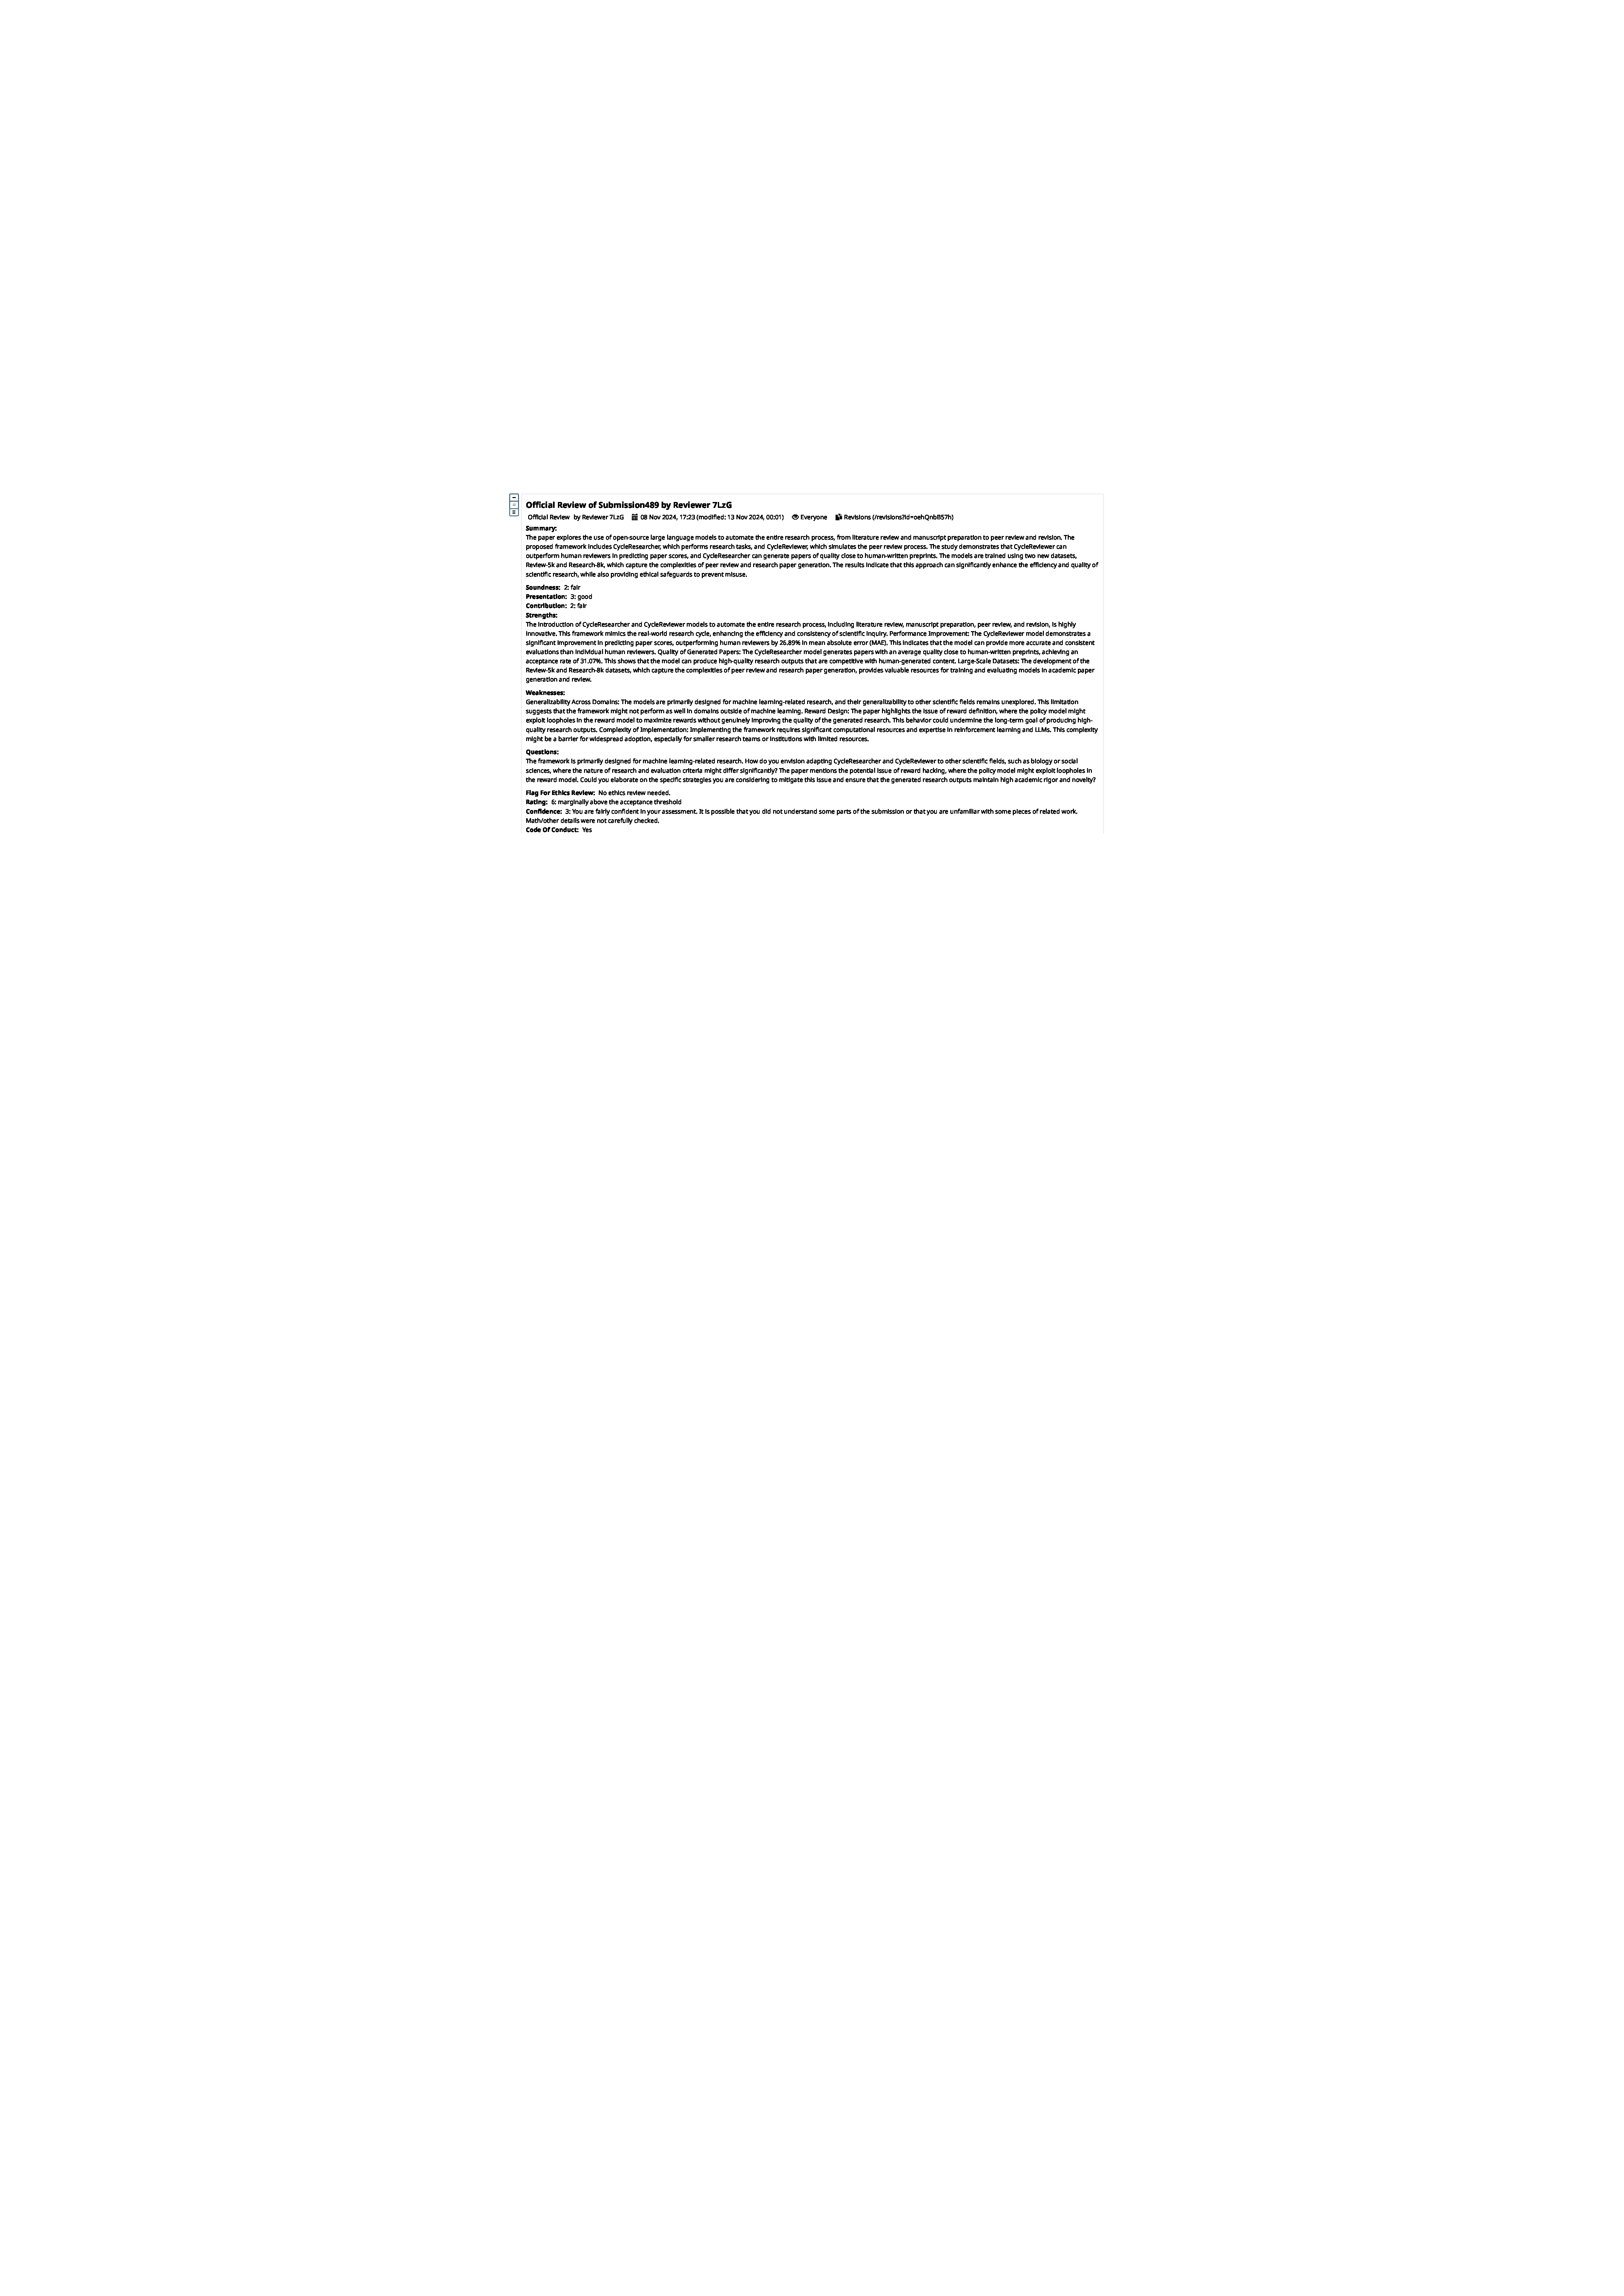
\includegraphics[width=\textwidth]{r1.pdf}
    \vspace{-0.3cm}
    \caption{The Real-world review comment for CycleResearcher}
    \vspace{-0.3cm}
    \label{fig:r1}
\end{figure*}

\begin{figure*}[t]
    \centering
    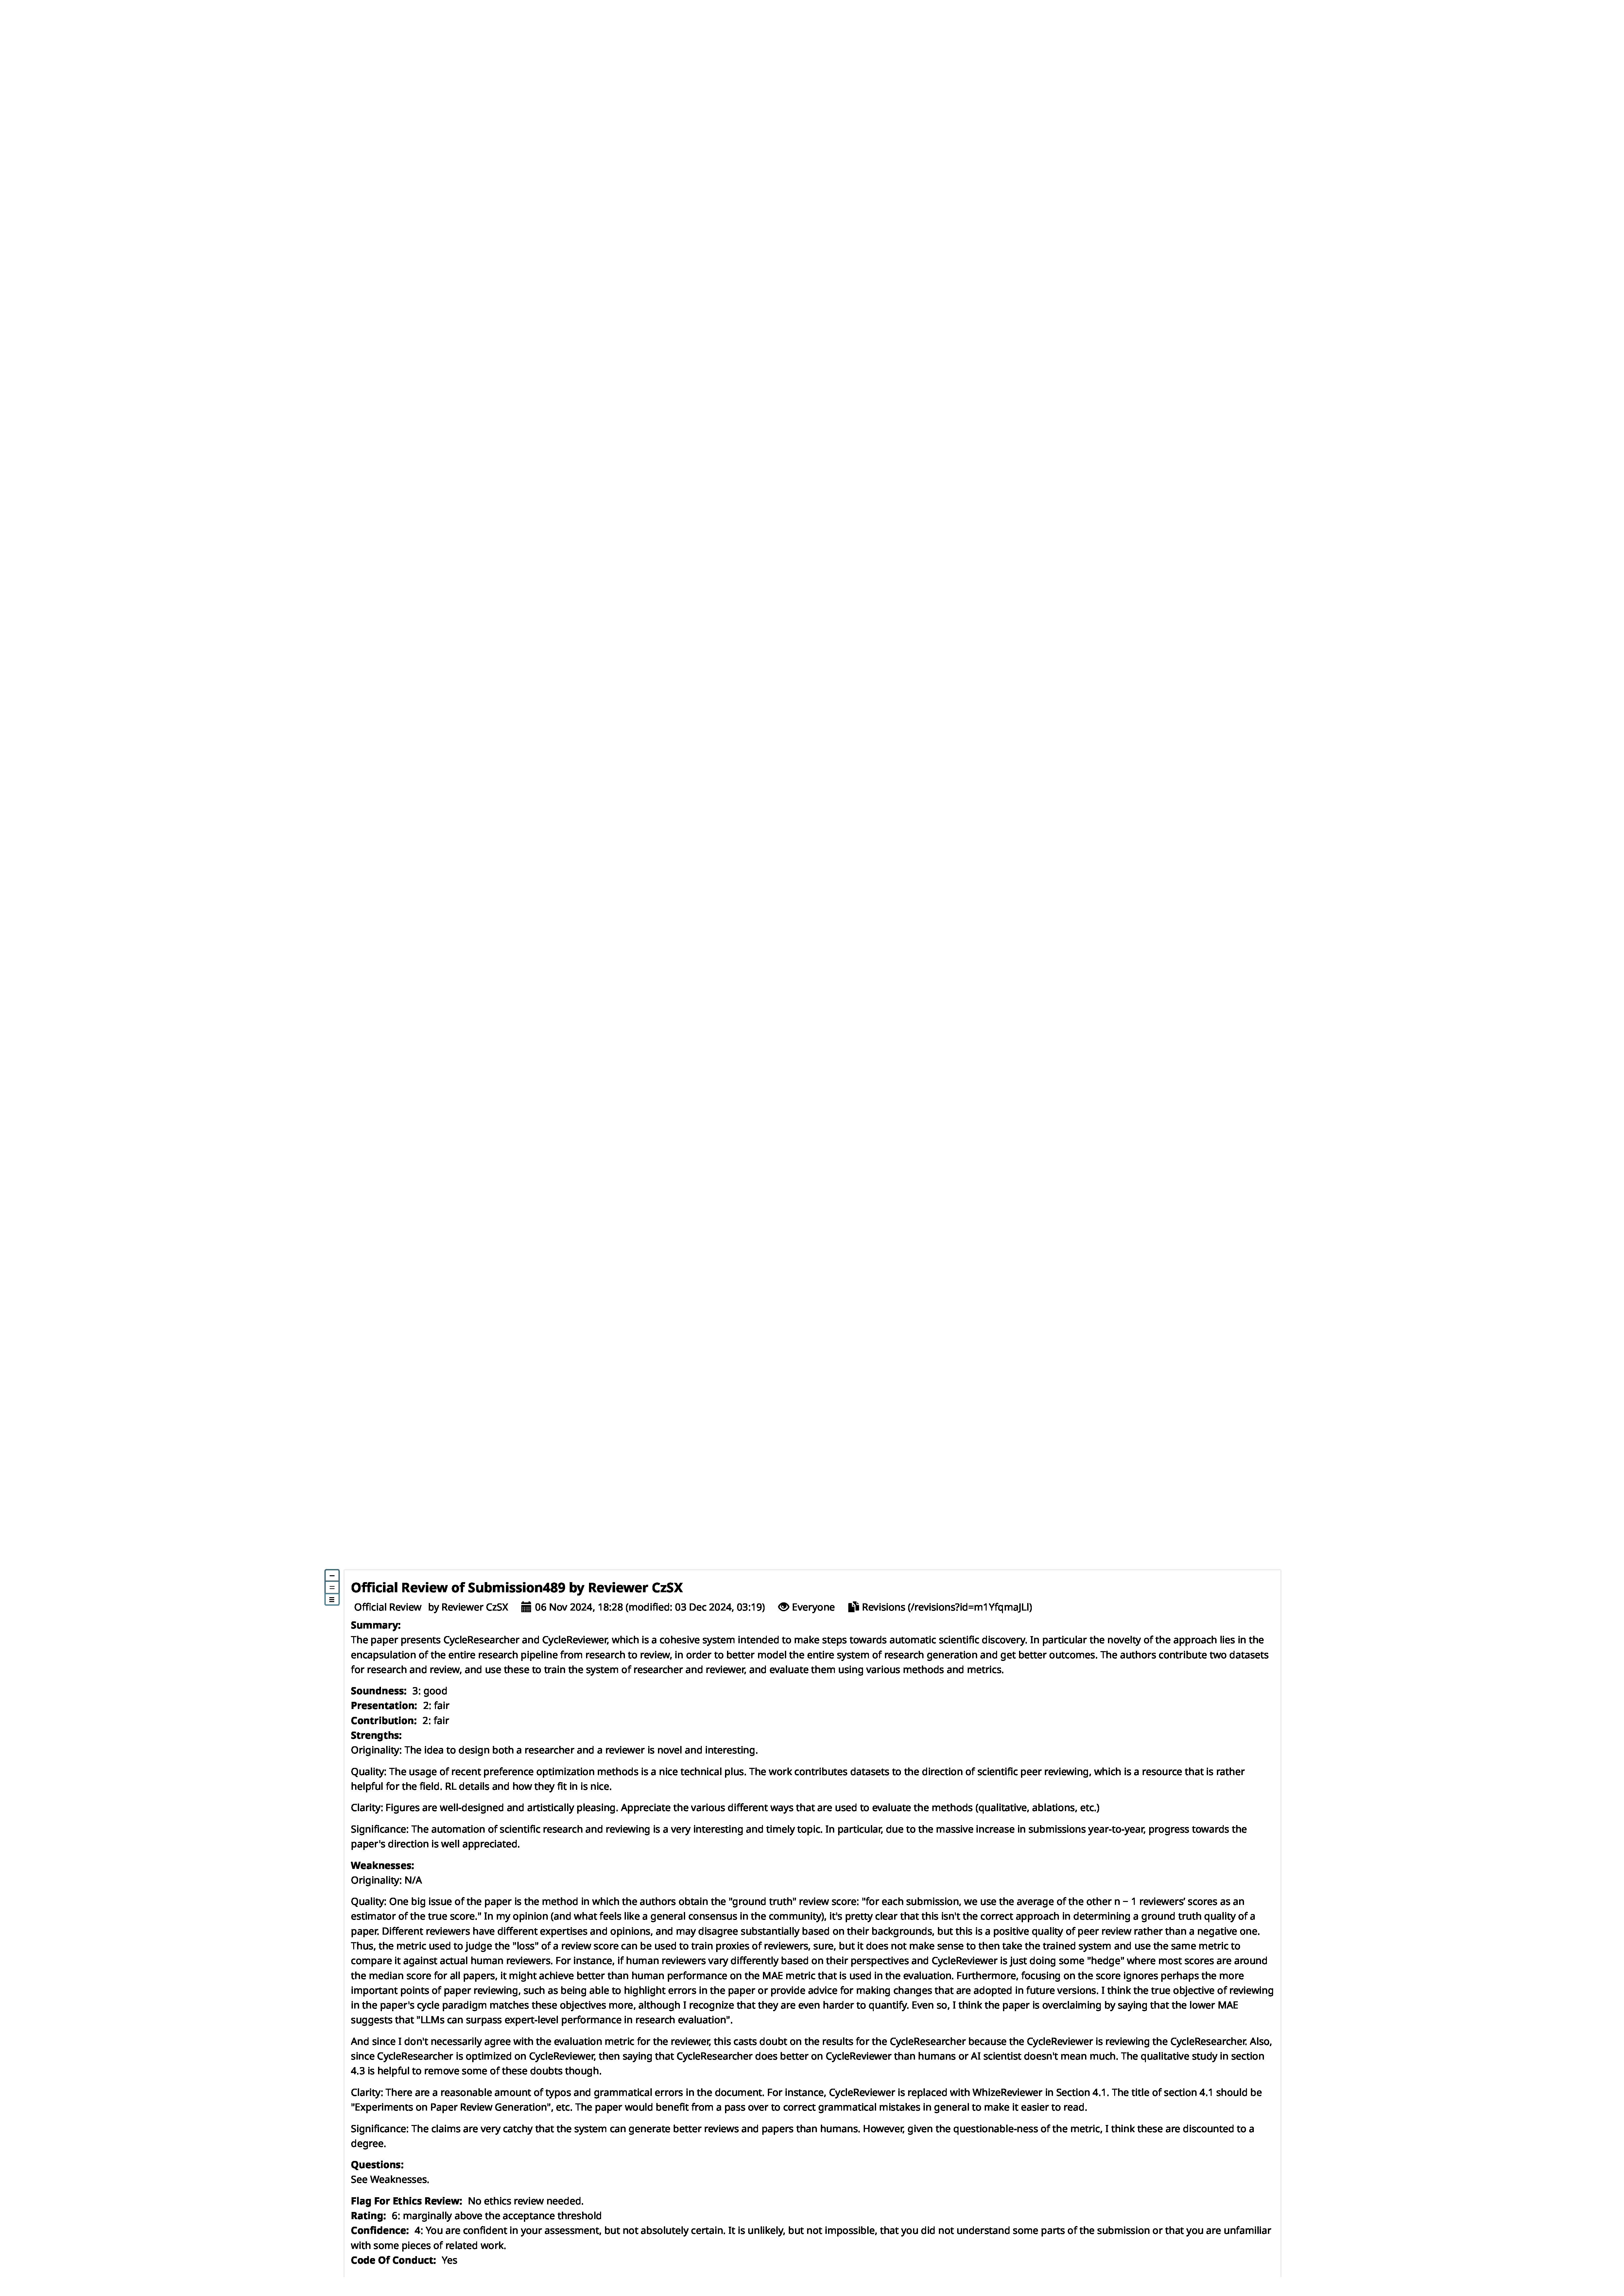
\includegraphics[width=0.86\textwidth]{r2.pdf}
    \vspace{-0.3cm}
    \caption{The Real-world review comment for CycleResearcher}
    \vspace{-0.3cm}
    \label{fig:r2}
\end{figure*}

\begin{figure*}[t]
    \centering
    
\includegraphics[width=0.8\textwidth]{r3.pdf}
    \vspace{-0.3cm}
    \caption{The Real-world review comment for CycleResearcher}
    \vspace{-0.3cm}
    \label{fig:r3}
\end{figure*}

\begin{figure*}[t]
    \centering
    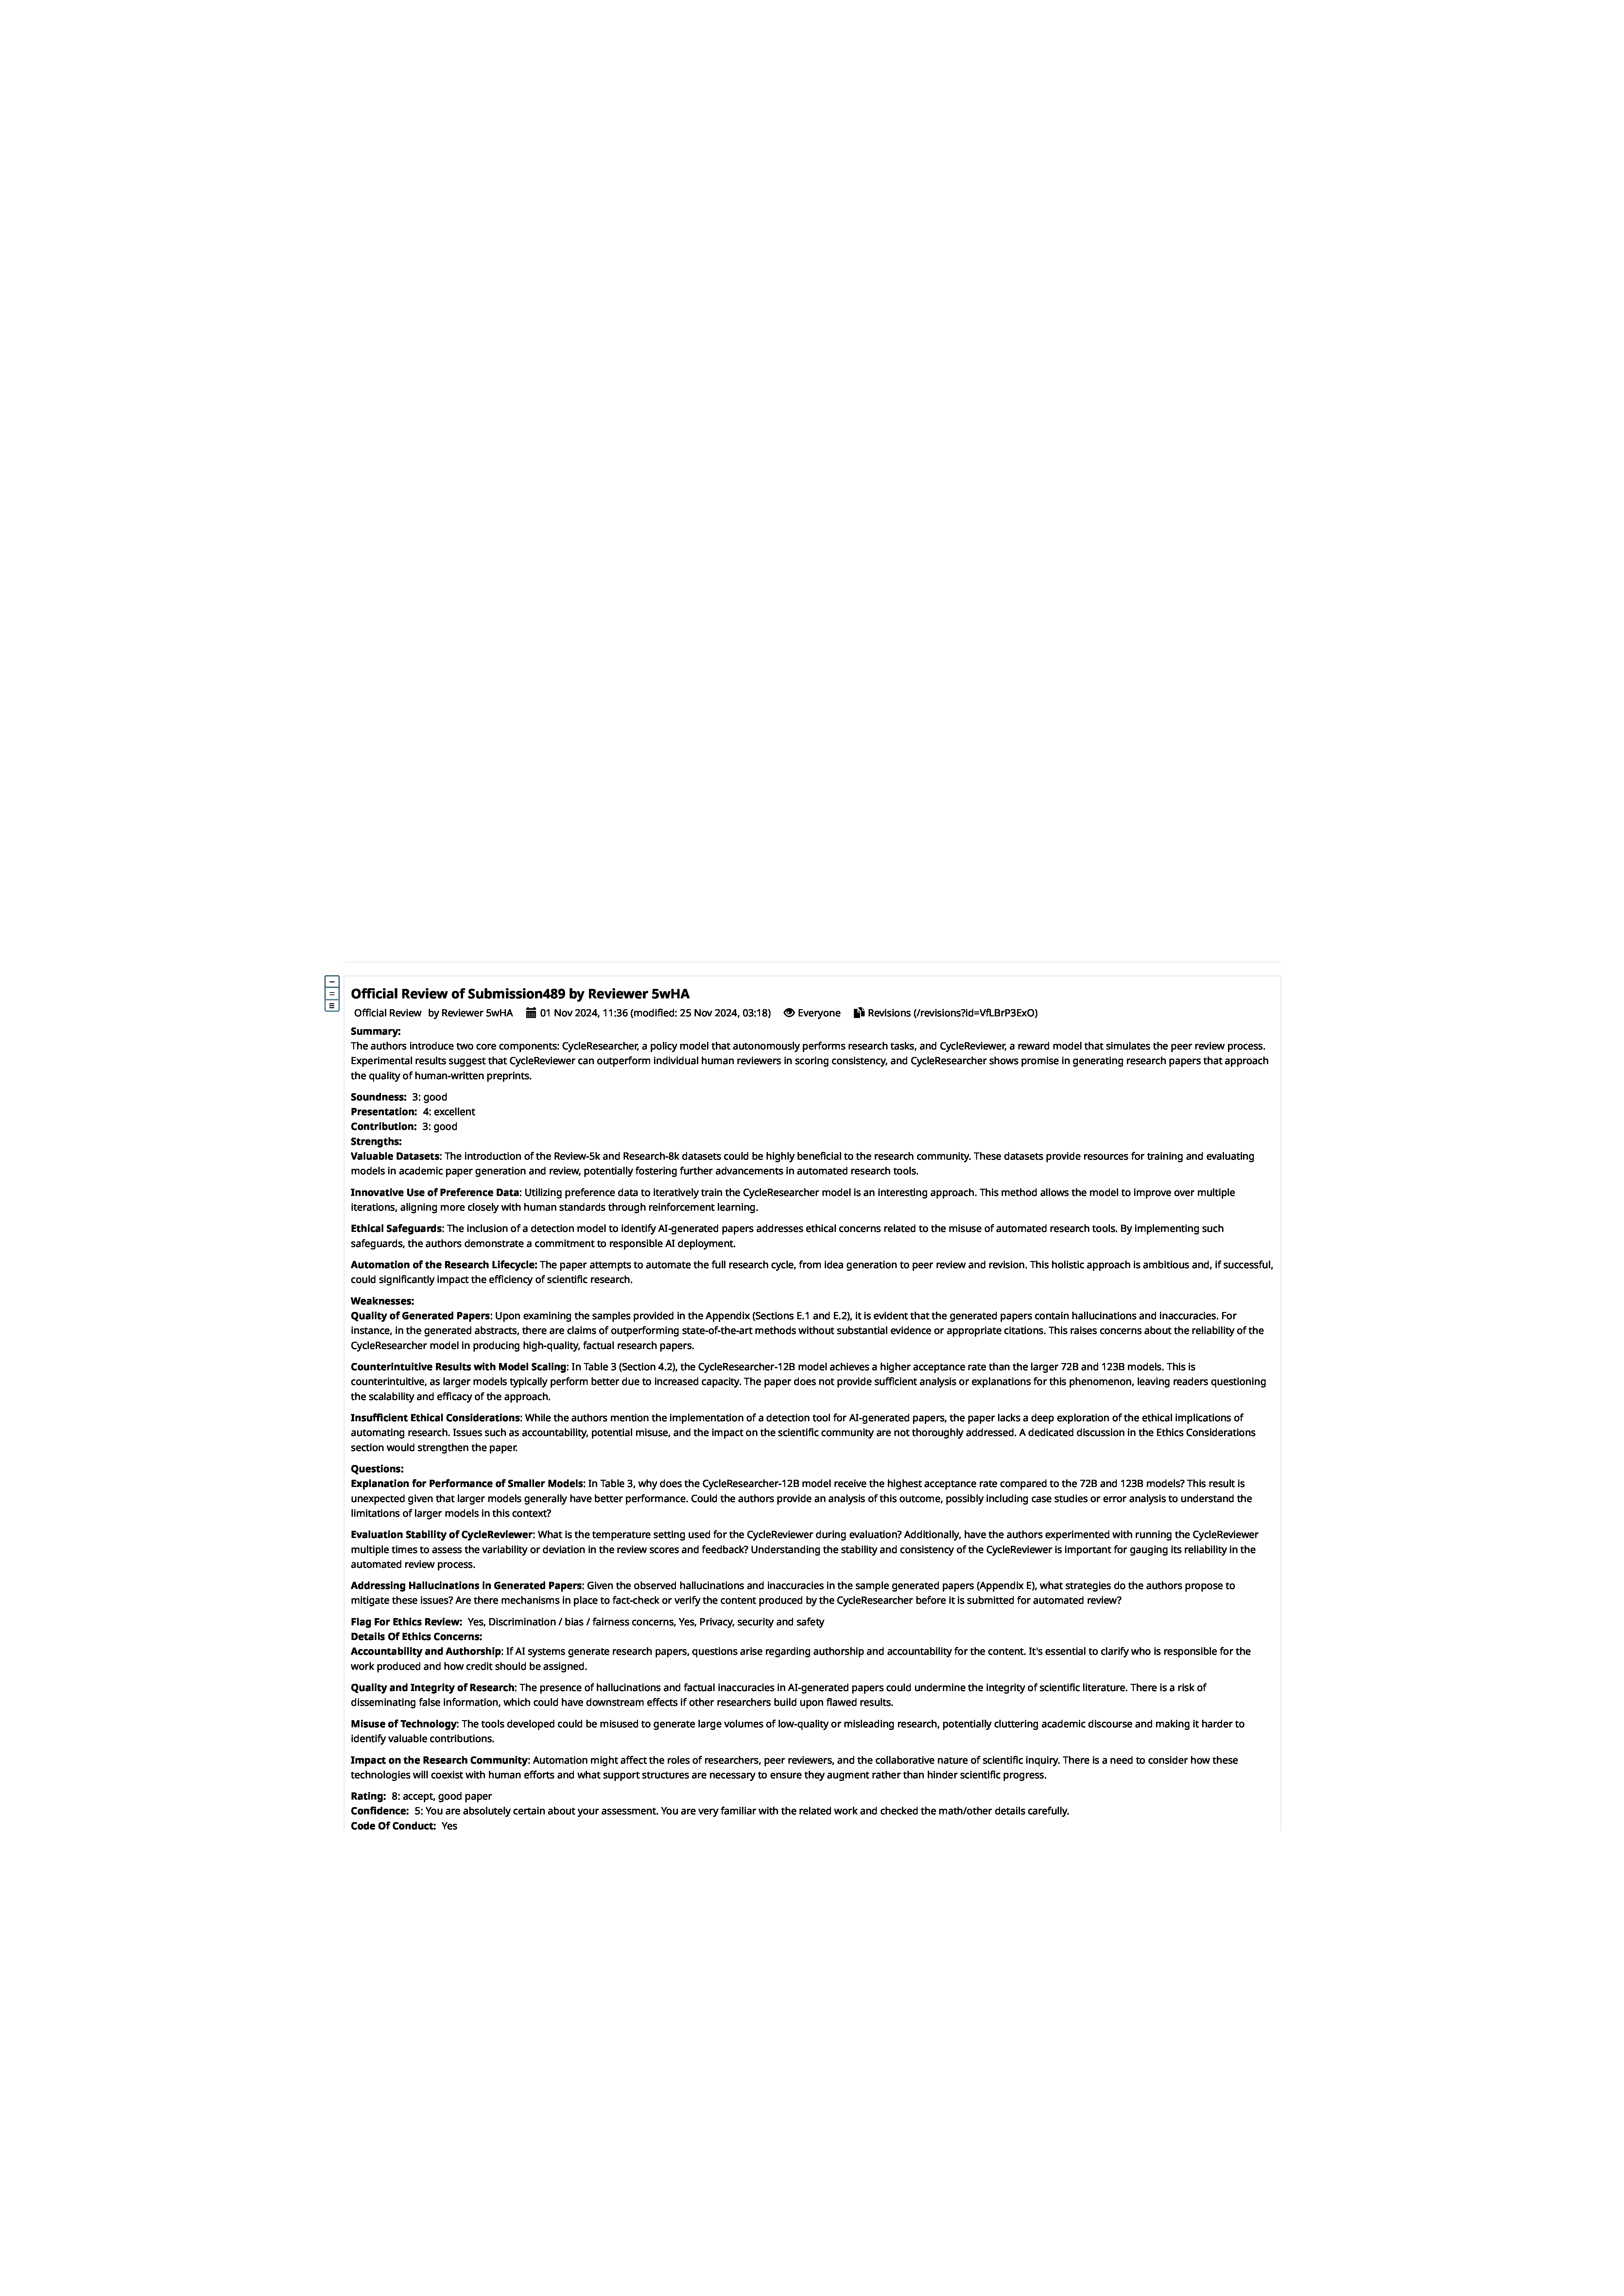
\includegraphics[width=0.72\textwidth]{r4.pdf}
    \vspace{-0.3cm}
    \caption{The Real-world review comment for CycleResearcher}
    \vspace{-0.3cm}
    \label{fig:r4}
\end{figure*}

\section{Information About Use Of AI Assistants}

This article has been reviewed by DeepReviewer-14B and revised accordingly based on its review comments.


\end{document}